\documentclass[twoside]{book}

% Packages required by doxygen
\usepackage{fixltx2e}
\usepackage{calc}
\usepackage{doxygen}
\usepackage[export]{adjustbox} % also loads graphicx
\usepackage{graphicx}
\usepackage[utf8]{inputenc}
\usepackage{makeidx}
\usepackage{multicol}
\usepackage{multirow}
\PassOptionsToPackage{warn}{textcomp}
\usepackage{textcomp}
\usepackage[nointegrals]{wasysym}
\usepackage[table]{xcolor}

% Font selection
\usepackage[T1]{fontenc}
\usepackage[scaled=.90]{helvet}
\usepackage{courier}
\usepackage{amssymb}
\usepackage{sectsty}
\renewcommand{\familydefault}{\sfdefault}
\allsectionsfont{%
  \fontseries{bc}\selectfont%
  \color{darkgray}%
}
\renewcommand{\DoxyLabelFont}{%
  \fontseries{bc}\selectfont%
  \color{darkgray}%
}
\newcommand{\+}{\discretionary{\mbox{\scriptsize$\hookleftarrow$}}{}{}}

% Page & text layout
\usepackage{geometry}
\geometry{%
  a4paper,%
  top=2.5cm,%
  bottom=2.5cm,%
  left=2.5cm,%
  right=2.5cm%
}
\tolerance=750
\hfuzz=15pt
\hbadness=750
\setlength{\emergencystretch}{15pt}
\setlength{\parindent}{0cm}
\setlength{\parskip}{3ex plus 2ex minus 2ex}
\makeatletter
\renewcommand{\paragraph}{%
  \@startsection{paragraph}{4}{0ex}{-1.0ex}{1.0ex}{%
    \normalfont\normalsize\bfseries\SS@parafont%
  }%
}
\renewcommand{\subparagraph}{%
  \@startsection{subparagraph}{5}{0ex}{-1.0ex}{1.0ex}{%
    \normalfont\normalsize\bfseries\SS@subparafont%
  }%
}
\makeatother

% Headers & footers
\usepackage{fancyhdr}
\pagestyle{fancyplain}
\fancyhead[LE]{\fancyplain{}{\bfseries\thepage}}
\fancyhead[CE]{\fancyplain{}{}}
\fancyhead[RE]{\fancyplain{}{\bfseries\leftmark}}
\fancyhead[LO]{\fancyplain{}{\bfseries\rightmark}}
\fancyhead[CO]{\fancyplain{}{}}
\fancyhead[RO]{\fancyplain{}{\bfseries\thepage}}
\fancyfoot[LE]{\fancyplain{}{}}
\fancyfoot[CE]{\fancyplain{}{}}
\fancyfoot[RE]{\fancyplain{}{\bfseries\scriptsize Generated by Doxygen }}
\fancyfoot[LO]{\fancyplain{}{\bfseries\scriptsize Generated by Doxygen }}
\fancyfoot[CO]{\fancyplain{}{}}
\fancyfoot[RO]{\fancyplain{}{}}
\renewcommand{\footrulewidth}{0.4pt}
\renewcommand{\chaptermark}[1]{%
  \markboth{#1}{}%
}
\renewcommand{\sectionmark}[1]{%
  \markright{\thesection\ #1}%
}

% Indices & bibliography
\usepackage{natbib}
\usepackage[titles]{tocloft}
\setcounter{tocdepth}{3}
\setcounter{secnumdepth}{5}
\makeindex

% Hyperlinks (required, but should be loaded last)
\usepackage{ifpdf}
\ifpdf
  \usepackage[pdftex,pagebackref=true]{hyperref}
\else
  \usepackage[ps2pdf,pagebackref=true]{hyperref}
\fi
\hypersetup{%
  colorlinks=true,%
  linkcolor=blue,%
  citecolor=blue,%
  unicode%
}

% Custom commands
\newcommand{\clearemptydoublepage}{%
  \newpage{\pagestyle{empty}\cleardoublepage}%
}

\usepackage{caption}
\captionsetup{labelsep=space,justification=centering,font={bf},singlelinecheck=off,skip=4pt,position=top}

%===== C O N T E N T S =====

\begin{document}

% Titlepage & ToC
\hypersetup{pageanchor=false,
             bookmarksnumbered=true,
             pdfencoding=unicode
            }
\pagenumbering{roman}
\begin{titlepage}
\vspace*{7cm}
\begin{center}%
{\Large Lane Detection }\\
\vspace*{1cm}
{\large Generated by Doxygen 1.8.11}\\
\end{center}
\end{titlepage}
\clearemptydoublepage
\tableofcontents
\clearemptydoublepage
\pagenumbering{arabic}
\hypersetup{pageanchor=true}

%--- Begin generated contents ---
\chapter{Hierarchical Index}
\section{Class Hierarchy}
This inheritance list is sorted roughly, but not completely, alphabetically\+:\begin{DoxyCompactList}
\item \contentsline{section}{Image\+Processing}{\pageref{classImageProcessing}}{}
\item \contentsline{section}{Lane\+Detection}{\pageref{classLaneDetection}}{}
\item \contentsline{section}{Lane\+Info}{\pageref{classLaneInfo}}{}
\item Test\begin{DoxyCompactList}
\item \contentsline{section}{Image\+Processing\+Test}{\pageref{classImageProcessingTest}}{}
\item \contentsline{section}{Lane\+Detection\+Test}{\pageref{classLaneDetectionTest}}{}
\item \contentsline{section}{Lane\+Info\+Test}{\pageref{classLaneInfoTest}}{}
\end{DoxyCompactList}
\end{DoxyCompactList}

\chapter{Class Index}
\section{Class List}
Here are the classes, structs, unions and interfaces with brief descriptions\+:\begin{DoxyCompactList}
\item\contentsline{section}{\hyperlink{classImageProcessing}{Image\+Processing} }{\pageref{classImageProcessing}}{}
\item\contentsline{section}{\hyperlink{classImageProcessingTest}{Image\+Processing\+Test} \\*Class to test \hyperlink{classImageProcessing}{Image\+Processing} }{\pageref{classImageProcessingTest}}{}
\item\contentsline{section}{\hyperlink{classLaneDetection}{Lane\+Detection} }{\pageref{classLaneDetection}}{}
\item\contentsline{section}{\hyperlink{classLaneDetectionTest}{Lane\+Detection\+Test} \\*Class to test \hyperlink{classLaneDetection}{Lane\+Detection} }{\pageref{classLaneDetectionTest}}{}
\item\contentsline{section}{\hyperlink{classLaneInfo}{Lane\+Info} }{\pageref{classLaneInfo}}{}
\item\contentsline{section}{\hyperlink{classLaneInfoTest}{Lane\+Info\+Test} \\*Class to test \hyperlink{classLaneInfo}{Lane\+Info} }{\pageref{classLaneInfoTest}}{}
\end{DoxyCompactList}

\chapter{File Index}
\section{File List}
Here is a list of all documented files with brief descriptions\+:\begin{DoxyCompactList}
\item\contentsline{section}{/home/akash/\+Lane\+Detection\+\_\+master/\+Lane\+Detection\+System/app/\hyperlink{ImageProcessing_8cpp}{Image\+Processing.\+cpp} \\*Image Processing Class File }{\pageref{ImageProcessing_8cpp}}{}
\item\contentsline{section}{/home/akash/\+Lane\+Detection\+\_\+master/\+Lane\+Detection\+System/app/\hyperlink{LaneDetection_8cpp}{Lane\+Detection.\+cpp} \\*Lane Detection Class file }{\pageref{LaneDetection_8cpp}}{}
\item\contentsline{section}{/home/akash/\+Lane\+Detection\+\_\+master/\+Lane\+Detection\+System/include/\hyperlink{ImageProcessing_8hpp}{Image\+Processing.\+hpp} \\*Image Processing Class Header }{\pageref{ImageProcessing_8hpp}}{}
\item\contentsline{section}{/home/akash/\+Lane\+Detection\+\_\+master/\+Lane\+Detection\+System/include/\hyperlink{LaneDetection_8hpp}{Lane\+Detection.\+hpp} \\*Lane Detection Class Header }{\pageref{LaneDetection_8hpp}}{}
\item\contentsline{section}{/home/akash/\+Lane\+Detection\+\_\+master/\+Lane\+Detection\+System/include/{\bfseries Lane\+Info.\+hpp} }{\pageref{LaneInfo_8hpp}}{}
\item\contentsline{section}{/home/akash/\+Lane\+Detection\+\_\+master/\+Lane\+Detection\+System/test/\hyperlink{ImageProcessingTest_8cpp}{Image\+Processing\+Test.\+cpp} \\*Image Processing Class Test }{\pageref{ImageProcessingTest_8cpp}}{}
\item\contentsline{section}{/home/akash/\+Lane\+Detection\+\_\+master/\+Lane\+Detection\+System/test/\hyperlink{LaneDetectionTest_8cpp}{Lane\+Detection\+Test.\+cpp} \\*Lane Detection Test }{\pageref{LaneDetectionTest_8cpp}}{}
\end{DoxyCompactList}

\chapter{Class Documentation}
\hypertarget{classImageProcessing}{}\section{Image\+Processing Class Reference}
\label{classImageProcessing}\index{Image\+Processing@{Image\+Processing}}
\subsection*{Public Member Functions}
\begin{DoxyCompactItemize}
\item 
\hyperlink{classImageProcessing_a0090ffe36a912d6df5d7a1f507f6252e}{Image\+Processing} ()
\begin{DoxyCompactList}\small\item\em Default constructor for Img\+Processing. \end{DoxyCompactList}\item 
virtual \hyperlink{classImageProcessing_a1d4bd00ec1862112552c663034cebabc}{$\sim$\+Image\+Processing} ()
\begin{DoxyCompactList}\small\item\em Default destructor for Img\+Processing. \end{DoxyCompactList}\item 
void \hyperlink{classImageProcessing_a72562595d5ec6974d5e4a715ac2c3f83}{pre\+Processing} (cv\+::\+Mat \&src, cv\+::\+Mat \&dst)
\begin{DoxyCompactList}\small\item\em Function to pre-\/process the input image. \end{DoxyCompactList}\item 
void \hyperlink{classImageProcessing_ab4520086fa3735882552ab376f94a9f8}{get\+Binary\+Img} (cv\+::\+Mat \&src, cv\+::\+Mat \&dst)
\begin{DoxyCompactList}\small\item\em Function to get a binary image after color thresholding and edge detection. \end{DoxyCompactList}\item 
void \hyperlink{classImageProcessing_aec91adad633adbbb0f0c0dc7fc595655}{prespective\+Transform} (cv\+::\+Mat \&src, cv\+::\+Mat \&dst, cv\+::\+Mat \&T\+\_\+perspective\+\_\+inv)
\begin{DoxyCompactList}\small\item\em Function to perform prospective transform. \end{DoxyCompactList}\item 
void \hyperlink{classImageProcessing_a0432eb5bac73ebc2d81442577f0466ef}{set\+Intrinsic} (double fx\+\_\+, double fy\+\_\+, double cx\+\_\+, double cy\+\_\+)
\begin{DoxyCompactList}\small\item\em Function to set camera matrix. \end{DoxyCompactList}\item 
void \hyperlink{classImageProcessing_a669c1fa1566fec74c944d8a74933bb8f}{set\+Dist\+Coeffs} (double k1\+\_\+, double k2\+\_\+, double p1\+\_\+, double p2\+\_\+, double k3\+\_\+)
\begin{DoxyCompactList}\small\item\em Function to set camera distortion. \end{DoxyCompactList}\item 
void \hyperlink{classImageProcessing_ade164d66f0f51ab799dbc949c03a7b57}{setgaussian\+SigmaX} (double gaussian\+Sigma\+X\+\_\+)
\begin{DoxyCompactList}\small\item\em Function to set standard deviation in X for gaussian blur. \end{DoxyCompactList}\item 
void \hyperlink{classImageProcessing_a4854cd009bb4ad04ab69e1ea701b71c8}{setgaussian\+SigmaY} (double gaussian\+Sigma\+Y\+\_\+)
\begin{DoxyCompactList}\small\item\em Function to set standard deviation in Y for gaussian blur. \end{DoxyCompactList}\item 
void \hyperlink{classImageProcessing_a748f92280f1a0773a56970b787a71682}{set\+Min\+Thresh\+H\+LS} (cv\+::\+Scalar min\+Thresh\+H\+S\+L\+\_\+)
\begin{DoxyCompactList}\small\item\em Function to set H\+SL color space minimum threshold value. \end{DoxyCompactList}\item 
void \hyperlink{classImageProcessing_a2595139a92ad3de27bcaab4a09d95ceb}{set\+Max\+Thresh\+H\+LS} (cv\+::\+Scalar max\+Thresh\+H\+S\+L\+\_\+)
\begin{DoxyCompactList}\small\item\em Function to set H\+SL color space maximum threshold value. \end{DoxyCompactList}\item 
void \hyperlink{classImageProcessing_a64b3a68e766210db6d7e6130d161acb6}{set\+Min\+Thresh\+B\+GR} (cv\+::\+Scalar min\+Thresh\+B\+G\+R\+\_\+)
\begin{DoxyCompactList}\small\item\em Function to set R\+GB color space minimum threshold value. \end{DoxyCompactList}\item 
void \hyperlink{classImageProcessing_ac11c15a2cbdbf71c6d6b1f10a768e4c2}{set\+Max\+Thresh\+B\+GR} (cv\+::\+Scalar max\+Thresh\+B\+G\+R\+\_\+)
\begin{DoxyCompactList}\small\item\em Function to set R\+GB color space maximum threshold value. \end{DoxyCompactList}\item 
cv\+::\+Mat \hyperlink{classImageProcessing_a3f38ff39191c4bec62e5ce03b5e72423}{get\+Intrinsic} (void)
\begin{DoxyCompactList}\small\item\em Function to get camera matrix. \end{DoxyCompactList}\item 
cv\+::\+Mat \hyperlink{classImageProcessing_a07b25ad0e2f707d451dd2cd905739c6d}{get\+Dist\+Coeffs} (void)
\begin{DoxyCompactList}\small\item\em Function to get camera distortion. \end{DoxyCompactList}\item 
double \hyperlink{classImageProcessing_aa0879ca32fc15e72d781723eb33de32e}{getgaussian\+SigmaX} (void)
\begin{DoxyCompactList}\small\item\em Function to get standard deviation in X for gaussian blur. \end{DoxyCompactList}\item 
double \hyperlink{classImageProcessing_a597f35362caec714d90e6a23be0db39c}{getgaussian\+SigmaY} (void)
\begin{DoxyCompactList}\small\item\em Function to get standard deviation in Y for gaussian blur. \end{DoxyCompactList}\item 
cv\+::\+Scalar \hyperlink{classImageProcessing_a08af88927411e7184e2efcebbf00ebf6}{get\+Min\+Thresh\+H\+LS} (void)
\begin{DoxyCompactList}\small\item\em Function to get H\+SL color space minimum threshold value. \end{DoxyCompactList}\item 
cv\+::\+Scalar \hyperlink{classImageProcessing_ab65db9a84fb0171397288951233511a2}{get\+Max\+Thresh\+H\+LS} (void)
\begin{DoxyCompactList}\small\item\em Function to get H\+SL color space maximum threshold value. \end{DoxyCompactList}\item 
cv\+::\+Scalar \hyperlink{classImageProcessing_a2ab2c6cc172c0d5bfed2123920b1fbec}{get\+Min\+Thresh\+B\+GR} (void)
\begin{DoxyCompactList}\small\item\em Function to get R\+GB color space minimum threshold value. \end{DoxyCompactList}\item 
cv\+::\+Scalar \hyperlink{classImageProcessing_a875d8972cdad191dc712f806d3795bae}{get\+Max\+Thresh\+B\+GR} (void)
\begin{DoxyCompactList}\small\item\em Function to get R\+GB color space maximum threshold value. \end{DoxyCompactList}\end{DoxyCompactItemize}


\subsection{Constructor \& Destructor Documentation}
\index{Image\+Processing@{Image\+Processing}!Image\+Processing@{Image\+Processing}}
\index{Image\+Processing@{Image\+Processing}!Image\+Processing@{Image\+Processing}}
\subsubsection[{\texorpdfstring{Image\+Processing()}{ImageProcessing()}}]{\setlength{\rightskip}{0pt plus 5cm}Image\+Processing\+::\+Image\+Processing (
\begin{DoxyParamCaption}
{}
\end{DoxyParamCaption}
)}\hypertarget{classImageProcessing_a0090ffe36a912d6df5d7a1f507f6252e}{}\label{classImageProcessing_a0090ffe36a912d6df5d7a1f507f6252e}


Default constructor for Img\+Processing. 


\begin{DoxyParams}{Parameters}
{\em nothing} & \\
\hline
\end{DoxyParams}
\begin{DoxyReturn}{Returns}
nothing 
\end{DoxyReturn}
\index{Image\+Processing@{Image\+Processing}!````~Image\+Processing@{$\sim$\+Image\+Processing}}
\index{````~Image\+Processing@{$\sim$\+Image\+Processing}!Image\+Processing@{Image\+Processing}}
\subsubsection[{\texorpdfstring{$\sim$\+Image\+Processing()}{~ImageProcessing()}}]{\setlength{\rightskip}{0pt plus 5cm}Image\+Processing\+::$\sim$\+Image\+Processing (
\begin{DoxyParamCaption}
{}
\end{DoxyParamCaption}
)\hspace{0.3cm}{\ttfamily [virtual]}}\hypertarget{classImageProcessing_a1d4bd00ec1862112552c663034cebabc}{}\label{classImageProcessing_a1d4bd00ec1862112552c663034cebabc}


Default destructor for Img\+Processing. 

Default destructor for \hyperlink{classImageProcessing}{Image\+Processing}.


\begin{DoxyParams}{Parameters}
{\em nothing} & \\
\hline
\end{DoxyParams}
\begin{DoxyReturn}{Returns}
nothing 
\end{DoxyReturn}


\subsection{Member Function Documentation}
\index{Image\+Processing@{Image\+Processing}!get\+Binary\+Img@{get\+Binary\+Img}}
\index{get\+Binary\+Img@{get\+Binary\+Img}!Image\+Processing@{Image\+Processing}}
\subsubsection[{\texorpdfstring{get\+Binary\+Img(cv\+::\+Mat \&src, cv\+::\+Mat \&dst)}{getBinaryImg(cv::Mat &src, cv::Mat &dst)}}]{\setlength{\rightskip}{0pt plus 5cm}void Image\+Processing\+::get\+Binary\+Img (
\begin{DoxyParamCaption}
\item[{cv\+::\+Mat \&}]{src, }
\item[{cv\+::\+Mat \&}]{dst}
\end{DoxyParamCaption}
)}\hypertarget{classImageProcessing_ab4520086fa3735882552ab376f94a9f8}{}\label{classImageProcessing_ab4520086fa3735882552ab376f94a9f8}


Function to get a binary image after color thresholding and edge detection. 


\begin{DoxyParams}{Parameters}
{\em masked} & image of type cv\+::\+Mat \\
\hline
{\em binary} & image of type cv\+::\+Mat \\
\hline
\end{DoxyParams}
\begin{DoxyReturn}{Returns}
nothing 
\end{DoxyReturn}
\index{Image\+Processing@{Image\+Processing}!get\+Dist\+Coeffs@{get\+Dist\+Coeffs}}
\index{get\+Dist\+Coeffs@{get\+Dist\+Coeffs}!Image\+Processing@{Image\+Processing}}
\subsubsection[{\texorpdfstring{get\+Dist\+Coeffs(void)}{getDistCoeffs(void)}}]{\setlength{\rightskip}{0pt plus 5cm}cv\+::\+Mat Image\+Processing\+::get\+Dist\+Coeffs (
\begin{DoxyParamCaption}
\item[{void}]{}
\end{DoxyParamCaption}
)}\hypertarget{classImageProcessing_a07b25ad0e2f707d451dd2cd905739c6d}{}\label{classImageProcessing_a07b25ad0e2f707d451dd2cd905739c6d}


Function to get camera distortion. 


\begin{DoxyParams}{Parameters}
{\em nothing} & \\
\hline
\end{DoxyParams}
\begin{DoxyReturn}{Returns}
distortion parameter k1 of type double distortion parameter k2 of type double distortion parameter p1 of type double distortion parameter p2 of type double distortion parameter k3 of type double 
\end{DoxyReturn}
\index{Image\+Processing@{Image\+Processing}!getgaussian\+SigmaX@{getgaussian\+SigmaX}}
\index{getgaussian\+SigmaX@{getgaussian\+SigmaX}!Image\+Processing@{Image\+Processing}}
\subsubsection[{\texorpdfstring{getgaussian\+Sigma\+X(void)}{getgaussianSigmaX(void)}}]{\setlength{\rightskip}{0pt plus 5cm}double Image\+Processing\+::getgaussian\+SigmaX (
\begin{DoxyParamCaption}
\item[{void}]{}
\end{DoxyParamCaption}
)}\hypertarget{classImageProcessing_aa0879ca32fc15e72d781723eb33de32e}{}\label{classImageProcessing_aa0879ca32fc15e72d781723eb33de32e}


Function to get standard deviation in X for gaussian blur. 


\begin{DoxyParams}{Parameters}
{\em nothing} & \\
\hline
\end{DoxyParams}
\begin{DoxyReturn}{Returns}
standard deviation in X for gaussian blur 
\end{DoxyReturn}
\index{Image\+Processing@{Image\+Processing}!getgaussian\+SigmaY@{getgaussian\+SigmaY}}
\index{getgaussian\+SigmaY@{getgaussian\+SigmaY}!Image\+Processing@{Image\+Processing}}
\subsubsection[{\texorpdfstring{getgaussian\+Sigma\+Y(void)}{getgaussianSigmaY(void)}}]{\setlength{\rightskip}{0pt plus 5cm}double Image\+Processing\+::getgaussian\+SigmaY (
\begin{DoxyParamCaption}
\item[{void}]{}
\end{DoxyParamCaption}
)}\hypertarget{classImageProcessing_a597f35362caec714d90e6a23be0db39c}{}\label{classImageProcessing_a597f35362caec714d90e6a23be0db39c}


Function to get standard deviation in Y for gaussian blur. 


\begin{DoxyParams}{Parameters}
{\em nothing} & \\
\hline
\end{DoxyParams}
\begin{DoxyReturn}{Returns}
standard deviation in Y for gaussian blur 
\end{DoxyReturn}
\index{Image\+Processing@{Image\+Processing}!get\+Intrinsic@{get\+Intrinsic}}
\index{get\+Intrinsic@{get\+Intrinsic}!Image\+Processing@{Image\+Processing}}
\subsubsection[{\texorpdfstring{get\+Intrinsic(void)}{getIntrinsic(void)}}]{\setlength{\rightskip}{0pt plus 5cm}cv\+::\+Mat Image\+Processing\+::get\+Intrinsic (
\begin{DoxyParamCaption}
\item[{void}]{}
\end{DoxyParamCaption}
)}\hypertarget{classImageProcessing_a3f38ff39191c4bec62e5ce03b5e72423}{}\label{classImageProcessing_a3f38ff39191c4bec62e5ce03b5e72423}


Function to get camera matrix. 


\begin{DoxyParams}{Parameters}
{\em nothing} & \\
\hline
\end{DoxyParams}
\begin{DoxyReturn}{Returns}
fx, the x component of focal length of type double fy, the y component of focal length of type double cx, the x coordinate of camera center of type double cy, the y coordinate of camera center of type double 
\end{DoxyReturn}
\index{Image\+Processing@{Image\+Processing}!get\+Max\+Thresh\+B\+GR@{get\+Max\+Thresh\+B\+GR}}
\index{get\+Max\+Thresh\+B\+GR@{get\+Max\+Thresh\+B\+GR}!Image\+Processing@{Image\+Processing}}
\subsubsection[{\texorpdfstring{get\+Max\+Thresh\+B\+G\+R(void)}{getMaxThreshBGR(void)}}]{\setlength{\rightskip}{0pt plus 5cm}cv\+::\+Scalar Image\+Processing\+::get\+Max\+Thresh\+B\+GR (
\begin{DoxyParamCaption}
\item[{void}]{}
\end{DoxyParamCaption}
)}\hypertarget{classImageProcessing_a875d8972cdad191dc712f806d3795bae}{}\label{classImageProcessing_a875d8972cdad191dc712f806d3795bae}


Function to get R\+GB color space maximum threshold value. 


\begin{DoxyParams}{Parameters}
{\em nothing} & \\
\hline
\end{DoxyParams}
\begin{DoxyReturn}{Returns}
maximum threshold values for red,green and blue, type cv\+::\+Vec$<$double, 3$>$ 
\end{DoxyReturn}
\index{Image\+Processing@{Image\+Processing}!get\+Max\+Thresh\+H\+LS@{get\+Max\+Thresh\+H\+LS}}
\index{get\+Max\+Thresh\+H\+LS@{get\+Max\+Thresh\+H\+LS}!Image\+Processing@{Image\+Processing}}
\subsubsection[{\texorpdfstring{get\+Max\+Thresh\+H\+L\+S(void)}{getMaxThreshHLS(void)}}]{\setlength{\rightskip}{0pt plus 5cm}cv\+::\+Scalar Image\+Processing\+::get\+Max\+Thresh\+H\+LS (
\begin{DoxyParamCaption}
\item[{void}]{}
\end{DoxyParamCaption}
)}\hypertarget{classImageProcessing_ab65db9a84fb0171397288951233511a2}{}\label{classImageProcessing_ab65db9a84fb0171397288951233511a2}


Function to get H\+SL color space maximum threshold value. 


\begin{DoxyParams}{Parameters}
{\em nothing} & \\
\hline
\end{DoxyParams}
\begin{DoxyReturn}{Returns}
maximum threshold values for hue,saturation and luminousness, type cv\+::\+Vec$<$double, 3$>$ 
\end{DoxyReturn}
\index{Image\+Processing@{Image\+Processing}!get\+Min\+Thresh\+B\+GR@{get\+Min\+Thresh\+B\+GR}}
\index{get\+Min\+Thresh\+B\+GR@{get\+Min\+Thresh\+B\+GR}!Image\+Processing@{Image\+Processing}}
\subsubsection[{\texorpdfstring{get\+Min\+Thresh\+B\+G\+R(void)}{getMinThreshBGR(void)}}]{\setlength{\rightskip}{0pt plus 5cm}cv\+::\+Scalar Image\+Processing\+::get\+Min\+Thresh\+B\+GR (
\begin{DoxyParamCaption}
\item[{void}]{}
\end{DoxyParamCaption}
)}\hypertarget{classImageProcessing_a2ab2c6cc172c0d5bfed2123920b1fbec}{}\label{classImageProcessing_a2ab2c6cc172c0d5bfed2123920b1fbec}


Function to get R\+GB color space minimum threshold value. 


\begin{DoxyParams}{Parameters}
{\em nothing} & \\
\hline
\end{DoxyParams}
\begin{DoxyReturn}{Returns}
minimum threshold values for red,green and blue, type cv\+::\+Vec$<$double, 3$>$ 
\end{DoxyReturn}
\index{Image\+Processing@{Image\+Processing}!get\+Min\+Thresh\+H\+LS@{get\+Min\+Thresh\+H\+LS}}
\index{get\+Min\+Thresh\+H\+LS@{get\+Min\+Thresh\+H\+LS}!Image\+Processing@{Image\+Processing}}
\subsubsection[{\texorpdfstring{get\+Min\+Thresh\+H\+L\+S(void)}{getMinThreshHLS(void)}}]{\setlength{\rightskip}{0pt plus 5cm}cv\+::\+Scalar Image\+Processing\+::get\+Min\+Thresh\+H\+LS (
\begin{DoxyParamCaption}
\item[{void}]{}
\end{DoxyParamCaption}
)}\hypertarget{classImageProcessing_a08af88927411e7184e2efcebbf00ebf6}{}\label{classImageProcessing_a08af88927411e7184e2efcebbf00ebf6}


Function to get H\+SL color space minimum threshold value. 


\begin{DoxyParams}{Parameters}
{\em nothing} & \\
\hline
\end{DoxyParams}
\begin{DoxyReturn}{Returns}
minimum threshold values for hue,saturation and luminousness, type cv\+::\+Vec$<$double, 3$>$
\end{DoxyReturn}

\begin{DoxyParams}{Parameters}
{\em nothing} & \\
\hline
\end{DoxyParams}
\begin{DoxyReturn}{Returns}
minimum threshold values for hue,saturation and luminousness, type cv\+::\+Vec$<$double, 3$>$ Function to get H\+SL color space minimum threshold value
\end{DoxyReturn}

\begin{DoxyParams}{Parameters}
{\em nothing} & \\
\hline
\end{DoxyParams}
\begin{DoxyReturn}{Returns}
minimum threshold values for hue,saturation and luminousness, type cv\+::\+Vec$<$double, 3$>$ 
\end{DoxyReturn}
\index{Image\+Processing@{Image\+Processing}!pre\+Processing@{pre\+Processing}}
\index{pre\+Processing@{pre\+Processing}!Image\+Processing@{Image\+Processing}}
\subsubsection[{\texorpdfstring{pre\+Processing(cv\+::\+Mat \&src, cv\+::\+Mat \&dst)}{preProcessing(cv::Mat &src, cv::Mat &dst)}}]{\setlength{\rightskip}{0pt plus 5cm}void Image\+Processing\+::pre\+Processing (
\begin{DoxyParamCaption}
\item[{cv\+::\+Mat \&}]{src, }
\item[{cv\+::\+Mat \&}]{dst}
\end{DoxyParamCaption}
)}\hypertarget{classImageProcessing_a72562595d5ec6974d5e4a715ac2c3f83}{}\label{classImageProcessing_a72562595d5ec6974d5e4a715ac2c3f83}


Function to pre-\/process the input image. 


\begin{DoxyParams}{Parameters}
{\em input} & image of type cv\+::\+Mat \\
\hline
{\em processed} & image of type cv\+::\+Mat \\
\hline
\end{DoxyParams}
\begin{DoxyReturn}{Returns}
nothing 
\end{DoxyReturn}
\index{Image\+Processing@{Image\+Processing}!prespective\+Transform@{prespective\+Transform}}
\index{prespective\+Transform@{prespective\+Transform}!Image\+Processing@{Image\+Processing}}
\subsubsection[{\texorpdfstring{prespective\+Transform(cv\+::\+Mat \&src, cv\+::\+Mat \&dst, cv\+::\+Mat \&\+T\+\_\+perspective\+\_\+inv)}{prespectiveTransform(cv::Mat &src, cv::Mat &dst, cv::Mat &T_perspective_inv)}}]{\setlength{\rightskip}{0pt plus 5cm}void Image\+Processing\+::prespective\+Transform (
\begin{DoxyParamCaption}
\item[{cv\+::\+Mat \&}]{src, }
\item[{cv\+::\+Mat \&}]{dst, }
\item[{cv\+::\+Mat \&}]{T\+\_\+perspective\+\_\+inv}
\end{DoxyParamCaption}
)}\hypertarget{classImageProcessing_aec91adad633adbbb0f0c0dc7fc595655}{}\label{classImageProcessing_aec91adad633adbbb0f0c0dc7fc595655}


Function to perform prospective transform. 


\begin{DoxyParams}{Parameters}
{\em binary} & image of type cv\+::\+Mat \\
\hline
{\em bird\textquotesingle{}s} & view image of type cv\+::\+Mat \\
\hline
\end{DoxyParams}
\begin{DoxyReturn}{Returns}
nothing 
\end{DoxyReturn}
\index{Image\+Processing@{Image\+Processing}!set\+Dist\+Coeffs@{set\+Dist\+Coeffs}}
\index{set\+Dist\+Coeffs@{set\+Dist\+Coeffs}!Image\+Processing@{Image\+Processing}}
\subsubsection[{\texorpdfstring{set\+Dist\+Coeffs(double k1\+\_\+, double k2\+\_\+, double p1\+\_\+, double p2\+\_\+, double k3\+\_\+)}{setDistCoeffs(double k1_, double k2_, double p1_, double p2_, double k3_)}}]{\setlength{\rightskip}{0pt plus 5cm}void Image\+Processing\+::set\+Dist\+Coeffs (
\begin{DoxyParamCaption}
\item[{double}]{k1\+\_\+, }
\item[{double}]{k2\+\_\+, }
\item[{double}]{p1\+\_\+, }
\item[{double}]{p2\+\_\+, }
\item[{double}]{k3\+\_\+}
\end{DoxyParamCaption}
)}\hypertarget{classImageProcessing_a669c1fa1566fec74c944d8a74933bb8f}{}\label{classImageProcessing_a669c1fa1566fec74c944d8a74933bb8f}


Function to set camera distortion. 


\begin{DoxyParams}{Parameters}
{\em distortion} & parameter k1 of type double \\
\hline
{\em distortion} & parameter k2 of type double \\
\hline
{\em distortion} & parameter p1 of type double \\
\hline
{\em distortion} & parameter p2 of type double \\
\hline
{\em distortion} & parameter k3 of type double \\
\hline
\end{DoxyParams}
\begin{DoxyReturn}{Returns}
nothing 
\end{DoxyReturn}
\index{Image\+Processing@{Image\+Processing}!setgaussian\+SigmaX@{setgaussian\+SigmaX}}
\index{setgaussian\+SigmaX@{setgaussian\+SigmaX}!Image\+Processing@{Image\+Processing}}
\subsubsection[{\texorpdfstring{setgaussian\+Sigma\+X(double gaussian\+Sigma\+X\+\_\+)}{setgaussianSigmaX(double gaussianSigmaX_)}}]{\setlength{\rightskip}{0pt plus 5cm}void Image\+Processing\+::setgaussian\+SigmaX (
\begin{DoxyParamCaption}
\item[{double}]{gaussian\+Sigma\+X\+\_\+}
\end{DoxyParamCaption}
)}\hypertarget{classImageProcessing_ade164d66f0f51ab799dbc949c03a7b57}{}\label{classImageProcessing_ade164d66f0f51ab799dbc949c03a7b57}


Function to set standard deviation in X for gaussian blur. 


\begin{DoxyParams}{Parameters}
{\em standard} & deviation in X for gaussian blur \\
\hline
\end{DoxyParams}
\begin{DoxyReturn}{Returns}
nothing 
\end{DoxyReturn}
\index{Image\+Processing@{Image\+Processing}!setgaussian\+SigmaY@{setgaussian\+SigmaY}}
\index{setgaussian\+SigmaY@{setgaussian\+SigmaY}!Image\+Processing@{Image\+Processing}}
\subsubsection[{\texorpdfstring{setgaussian\+Sigma\+Y(double gaussian\+Sigma\+Y\+\_\+)}{setgaussianSigmaY(double gaussianSigmaY_)}}]{\setlength{\rightskip}{0pt plus 5cm}void Image\+Processing\+::setgaussian\+SigmaY (
\begin{DoxyParamCaption}
\item[{double}]{gaussian\+Sigma\+Y\+\_\+}
\end{DoxyParamCaption}
)}\hypertarget{classImageProcessing_a4854cd009bb4ad04ab69e1ea701b71c8}{}\label{classImageProcessing_a4854cd009bb4ad04ab69e1ea701b71c8}


Function to set standard deviation in Y for gaussian blur. 


\begin{DoxyParams}{Parameters}
{\em standard} & deviation in Y for gaussian blur \\
\hline
\end{DoxyParams}
\begin{DoxyReturn}{Returns}
nothing 
\end{DoxyReturn}
\index{Image\+Processing@{Image\+Processing}!set\+Intrinsic@{set\+Intrinsic}}
\index{set\+Intrinsic@{set\+Intrinsic}!Image\+Processing@{Image\+Processing}}
\subsubsection[{\texorpdfstring{set\+Intrinsic(double fx\+\_\+, double fy\+\_\+, double cx\+\_\+, double cy\+\_\+)}{setIntrinsic(double fx_, double fy_, double cx_, double cy_)}}]{\setlength{\rightskip}{0pt plus 5cm}void Image\+Processing\+::set\+Intrinsic (
\begin{DoxyParamCaption}
\item[{double}]{fx\+\_\+, }
\item[{double}]{fy\+\_\+, }
\item[{double}]{cx\+\_\+, }
\item[{double}]{cy\+\_\+}
\end{DoxyParamCaption}
)}\hypertarget{classImageProcessing_a0432eb5bac73ebc2d81442577f0466ef}{}\label{classImageProcessing_a0432eb5bac73ebc2d81442577f0466ef}


Function to set camera matrix. 


\begin{DoxyParams}{Parameters}
{\em fx,the} & x component of focal length of type double \\
\hline
{\em fy,the} & y component of focal length of type double \\
\hline
{\em cx,the} & x coordinate of camera center of type double \\
\hline
{\em cy,the} & y coordinate of camera center of type double \\
\hline
\end{DoxyParams}
\begin{DoxyReturn}{Returns}
nothing 
\end{DoxyReturn}
\index{Image\+Processing@{Image\+Processing}!set\+Max\+Thresh\+B\+GR@{set\+Max\+Thresh\+B\+GR}}
\index{set\+Max\+Thresh\+B\+GR@{set\+Max\+Thresh\+B\+GR}!Image\+Processing@{Image\+Processing}}
\subsubsection[{\texorpdfstring{set\+Max\+Thresh\+B\+G\+R(cv\+::\+Scalar max\+Thresh\+B\+G\+R\+\_\+)}{setMaxThreshBGR(cv::Scalar maxThreshBGR_)}}]{\setlength{\rightskip}{0pt plus 5cm}void Image\+Processing\+::set\+Max\+Thresh\+B\+GR (
\begin{DoxyParamCaption}
\item[{cv\+::\+Scalar}]{max\+Thresh\+B\+G\+R\+\_\+}
\end{DoxyParamCaption}
)}\hypertarget{classImageProcessing_ac11c15a2cbdbf71c6d6b1f10a768e4c2}{}\label{classImageProcessing_ac11c15a2cbdbf71c6d6b1f10a768e4c2}


Function to set R\+GB color space maximum threshold value. 


\begin{DoxyParams}{Parameters}
{\em maximum} & threshold values for red,green and blue, type cv\+::\+Vec$<$double, 3$>$ \\
\hline
\end{DoxyParams}
\begin{DoxyReturn}{Returns}
nothing 
\end{DoxyReturn}
\index{Image\+Processing@{Image\+Processing}!set\+Max\+Thresh\+H\+LS@{set\+Max\+Thresh\+H\+LS}}
\index{set\+Max\+Thresh\+H\+LS@{set\+Max\+Thresh\+H\+LS}!Image\+Processing@{Image\+Processing}}
\subsubsection[{\texorpdfstring{set\+Max\+Thresh\+H\+L\+S(cv\+::\+Scalar max\+Thresh\+H\+S\+L\+\_\+)}{setMaxThreshHLS(cv::Scalar maxThreshHSL_)}}]{\setlength{\rightskip}{0pt plus 5cm}void Image\+Processing\+::set\+Max\+Thresh\+H\+LS (
\begin{DoxyParamCaption}
\item[{cv\+::\+Scalar}]{max\+Thresh\+H\+L\+S\+\_\+}
\end{DoxyParamCaption}
)}\hypertarget{classImageProcessing_a2595139a92ad3de27bcaab4a09d95ceb}{}\label{classImageProcessing_a2595139a92ad3de27bcaab4a09d95ceb}


Function to set H\+SL color space maximum threshold value. 


\begin{DoxyParams}{Parameters}
{\em maximum} & threshold values for hue,saturation and luminousness, type cv\+::\+Vec$<$double, 3$>$ \\
\hline
\end{DoxyParams}
\begin{DoxyReturn}{Returns}
nothing 
\end{DoxyReturn}
\index{Image\+Processing@{Image\+Processing}!set\+Min\+Thresh\+B\+GR@{set\+Min\+Thresh\+B\+GR}}
\index{set\+Min\+Thresh\+B\+GR@{set\+Min\+Thresh\+B\+GR}!Image\+Processing@{Image\+Processing}}
\subsubsection[{\texorpdfstring{set\+Min\+Thresh\+B\+G\+R(cv\+::\+Scalar min\+Thresh\+B\+G\+R\+\_\+)}{setMinThreshBGR(cv::Scalar minThreshBGR_)}}]{\setlength{\rightskip}{0pt plus 5cm}void Image\+Processing\+::set\+Min\+Thresh\+B\+GR (
\begin{DoxyParamCaption}
\item[{cv\+::\+Scalar}]{min\+Thresh\+B\+G\+R\+\_\+}
\end{DoxyParamCaption}
)}\hypertarget{classImageProcessing_a64b3a68e766210db6d7e6130d161acb6}{}\label{classImageProcessing_a64b3a68e766210db6d7e6130d161acb6}


Function to set R\+GB color space minimum threshold value. 


\begin{DoxyParams}{Parameters}
{\em minimum} & threshold values for red,green and blue, type cv\+::\+Vec$<$double, 3$>$ \\
\hline
\end{DoxyParams}
\begin{DoxyReturn}{Returns}
nothing 
\end{DoxyReturn}
\index{Image\+Processing@{Image\+Processing}!set\+Min\+Thresh\+H\+LS@{set\+Min\+Thresh\+H\+LS}}
\index{set\+Min\+Thresh\+H\+LS@{set\+Min\+Thresh\+H\+LS}!Image\+Processing@{Image\+Processing}}
\subsubsection[{\texorpdfstring{set\+Min\+Thresh\+H\+L\+S(cv\+::\+Scalar min\+Thresh\+H\+S\+L\+\_\+)}{setMinThreshHLS(cv::Scalar minThreshHSL_)}}]{\setlength{\rightskip}{0pt plus 5cm}void Image\+Processing\+::set\+Min\+Thresh\+H\+LS (
\begin{DoxyParamCaption}
\item[{cv\+::\+Scalar}]{min\+Thresh\+H\+L\+S\+\_\+}
\end{DoxyParamCaption}
)}\hypertarget{classImageProcessing_a748f92280f1a0773a56970b787a71682}{}\label{classImageProcessing_a748f92280f1a0773a56970b787a71682}


Function to set H\+SL color space minimum threshold value. 


\begin{DoxyParams}{Parameters}
{\em minimum} & threshold values for hue,saturation and luminousness, type cv\+::\+Vec$<$double, 3$>$ \\
\hline
\end{DoxyParams}
\begin{DoxyReturn}{Returns}
nothing 
\end{DoxyReturn}


The documentation for this class was generated from the following files\+:\begin{DoxyCompactItemize}
\item 
/home/akash/\+Lane\+Detection\+\_\+master/\+Lane\+Detection\+System/include/\hyperlink{ImageProcessing_8hpp}{Image\+Processing.\+hpp}\item 
/home/akash/\+Lane\+Detection\+\_\+master/\+Lane\+Detection\+System/app/\hyperlink{ImageProcessing_8cpp}{Image\+Processing.\+cpp}\end{DoxyCompactItemize}

\hypertarget{classImageProcessingTest}{}\section{Image\+Processing\+Test Class Reference}
\label{classImageProcessingTest}\index{Image\+Processing\+Test@{Image\+Processing\+Test}}


Class to test \hyperlink{classImageProcessing}{Image\+Processing}.  




Inheritance diagram for Image\+Processing\+Test\+:
\nopagebreak
\begin{figure}[H]
\begin{center}
\leavevmode
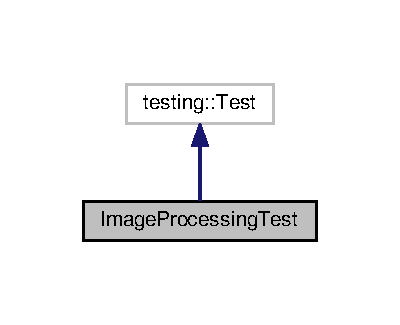
\includegraphics[width=192pt]{classImageProcessingTest__inherit__graph}
\end{center}
\end{figure}


Collaboration diagram for Image\+Processing\+Test\+:
\nopagebreak
\begin{figure}[H]
\begin{center}
\leavevmode
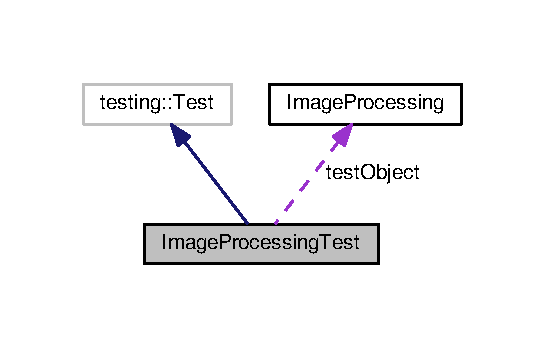
\includegraphics[width=262pt]{classImageProcessingTest__coll__graph}
\end{center}
\end{figure}
\subsection*{Protected Attributes}
\begin{DoxyCompactItemize}
\item 
\hyperlink{classImageProcessing}{Image\+Processing} {\bfseries test\+Object}\hypertarget{classImageProcessingTest_a209398691b93a4f2d8482fc7b642c5e4}{}\label{classImageProcessingTest_a209398691b93a4f2d8482fc7b642c5e4}

\end{DoxyCompactItemize}


\subsection{Detailed Description}
Class to test \hyperlink{classImageProcessing}{Image\+Processing}. 

The documentation for this class was generated from the following file\+:\begin{DoxyCompactItemize}
\item 
/home/akash/\+Lane\+Detection\+\_\+master/\+Lane\+Detection\+System/test/\hyperlink{ImageProcessingTest_8cpp}{Image\+Processing\+Test.\+cpp}\end{DoxyCompactItemize}

\hypertarget{classLaneDetection}{}\section{Lane\+Detection Class Reference}
\label{classLaneDetection}\index{Lane\+Detection@{Lane\+Detection}}
\subsection*{Public Member Functions}
\begin{DoxyCompactItemize}
\item 
\hyperlink{classLaneDetection_a731f54ebd16a6ad77ff51e413415d1d9}{Lane\+Detection} ()
\begin{DoxyCompactList}\small\item\em Default constructor for \hyperlink{classLaneDetection}{Lane\+Detection}. \end{DoxyCompactList}\item 
\hyperlink{classLaneDetection_afdccabf18bc0137fafb973624e8c3df3}{$\sim$\+Lane\+Detection} ()
\begin{DoxyCompactList}\small\item\em Default destructor for \hyperlink{classLaneDetection}{Lane\+Detection}. \end{DoxyCompactList}\item 
void \hyperlink{classLaneDetection_a543e9a9346892343830f0641613e330a}{generate\+Hist} (cv\+::\+Mat \&src, std\+::vector$<$ double $>$ \&hist)
\begin{DoxyCompactList}\small\item\em Function to generate lane pixel histogram. \end{DoxyCompactList}\item 
int \hyperlink{classLaneDetection_a3291cc176ecd5d81cb0e778741c7bad7}{average\+Window\+Center} (int \&x\+Val)
\begin{DoxyCompactList}\small\item\em Function to get average of window center. \end{DoxyCompactList}\item 
void \hyperlink{classLaneDetection_accd042559d371231d11544b341b2fa66}{extract\+Lane} (cv\+::\+Mat \&perspective\+Img, std\+::vector$<$ double $>$ \&hist, std\+::vector$<$ cv\+::\+Point $>$ \&dst\+Lane, std\+::string lane\+Type, cv\+::\+Mat \&draw\+Window)
\begin{DoxyCompactList}\small\item\em Function to extract left or right lane. \end{DoxyCompactList}\item 
void \hyperlink{classLaneDetection_aafdb4913fa1ce44bd272c7c6c82b7885}{fit\+Poly} (std\+::vector$<$ cv\+::\+Point $>$ \&lane\+LR, cv\+::\+Mat \&dst\+Lane\+Parameters, int order)
\begin{DoxyCompactList}\small\item\em Function to fit a polynomial on the received lane pixel data. \end{DoxyCompactList}\item 
void \hyperlink{classLaneDetection_a222e9cc724b5a9a7bc1ffbfd66bf77aa}{extract\+Central\+Line} (std\+::vector$<$ cv\+::\+Point $>$ \&left\+Lane\+Points, std\+::vector$<$ cv\+::\+Point $>$ \&central\+Line)
\begin{DoxyCompactList}\small\item\em Function to extract central line. \end{DoxyCompactList}\item 
double \hyperlink{classLaneDetection_af8a40b3f7afe04c2688bed7d7cd13319}{compute\+Turn\+Angle} (std\+::vector$<$ cv\+::\+Point $>$ \&left\+Line)
\begin{DoxyCompactList}\small\item\em Function to compute turn angle for the lane. \end{DoxyCompactList}\item 
void \hyperlink{classLaneDetection_a6c89cf64d45414120997d724bcf3a2a8}{detect\+Lanes} (void)
\begin{DoxyCompactList}\small\item\em Function to implement the entire system pipeline. \end{DoxyCompactList}\end{DoxyCompactItemize}


\subsection{Constructor \& Destructor Documentation}
\index{Lane\+Detection@{Lane\+Detection}!Lane\+Detection@{Lane\+Detection}}
\index{Lane\+Detection@{Lane\+Detection}!Lane\+Detection@{Lane\+Detection}}
\subsubsection[{\texorpdfstring{Lane\+Detection()}{LaneDetection()}}]{\setlength{\rightskip}{0pt plus 5cm}Lane\+Detection\+::\+Lane\+Detection (
\begin{DoxyParamCaption}
{}
\end{DoxyParamCaption}
)}\hypertarget{classLaneDetection_a731f54ebd16a6ad77ff51e413415d1d9}{}\label{classLaneDetection_a731f54ebd16a6ad77ff51e413415d1d9}


Default constructor for \hyperlink{classLaneDetection}{Lane\+Detection}. 


\begin{DoxyParams}{Parameters}
{\em nothing} & \\
\hline
\end{DoxyParams}
\begin{DoxyReturn}{Returns}
nothing 
\end{DoxyReturn}
\index{Lane\+Detection@{Lane\+Detection}!````~Lane\+Detection@{$\sim$\+Lane\+Detection}}
\index{````~Lane\+Detection@{$\sim$\+Lane\+Detection}!Lane\+Detection@{Lane\+Detection}}
\subsubsection[{\texorpdfstring{$\sim$\+Lane\+Detection()}{~LaneDetection()}}]{\setlength{\rightskip}{0pt plus 5cm}Lane\+Detection\+::$\sim$\+Lane\+Detection (
\begin{DoxyParamCaption}
{}
\end{DoxyParamCaption}
)}\hypertarget{classLaneDetection_afdccabf18bc0137fafb973624e8c3df3}{}\label{classLaneDetection_afdccabf18bc0137fafb973624e8c3df3}


Default destructor for \hyperlink{classLaneDetection}{Lane\+Detection}. 


\begin{DoxyParams}{Parameters}
{\em nothing} & \\
\hline
\end{DoxyParams}
\begin{DoxyReturn}{Returns}
nothing
\end{DoxyReturn}

\begin{DoxyParams}{Parameters}
{\em } & \\
\hline
\end{DoxyParams}


\subsection{Member Function Documentation}
\index{Lane\+Detection@{Lane\+Detection}!average\+Window\+Center@{average\+Window\+Center}}
\index{average\+Window\+Center@{average\+Window\+Center}!Lane\+Detection@{Lane\+Detection}}
\subsubsection[{\texorpdfstring{average\+Window\+Center(int \&x\+Val)}{averageWindowCenter(int &xVal)}}]{\setlength{\rightskip}{0pt plus 5cm}int Lane\+Detection\+::average\+Window\+Center (
\begin{DoxyParamCaption}
\item[{int \&}]{x\+Val\+\_\+}
\end{DoxyParamCaption}
)}\hypertarget{classLaneDetection_a3291cc176ecd5d81cb0e778741c7bad7}{}\label{classLaneDetection_a3291cc176ecd5d81cb0e778741c7bad7}


Function to get average of window center. 


\begin{DoxyParams}{Parameters}
{\em histogram} & containing lane pixels of type cv\+::\+Mat \\
\hline
{\em pixel} & locations of left or right lane, type std\+::vector$<$cv\+::\+Point\+\_\+$<$int$>$$>$ \\
\hline
{\em lane} & to be extracted -\/ left or right of type string \\
\hline
\end{DoxyParams}
\begin{DoxyReturn}{Returns}
nothing 
\end{DoxyReturn}
\index{Lane\+Detection@{Lane\+Detection}!compute\+Turn\+Angle@{compute\+Turn\+Angle}}
\index{compute\+Turn\+Angle@{compute\+Turn\+Angle}!Lane\+Detection@{Lane\+Detection}}
\subsubsection[{\texorpdfstring{compute\+Turn\+Angle(std\+::vector$<$ cv\+::\+Point $>$ \&left\+Line)}{computeTurnAngle(std::vector< cv::Point > &leftLine)}}]{\setlength{\rightskip}{0pt plus 5cm}double Lane\+Detection\+::compute\+Turn\+Angle (
\begin{DoxyParamCaption}
\item[{std\+::vector$<$ cv\+::\+Point $>$ \&}]{left\+Line}
\end{DoxyParamCaption}
)}\hypertarget{classLaneDetection_af8a40b3f7afe04c2688bed7d7cd13319}{}\label{classLaneDetection_af8a40b3f7afe04c2688bed7d7cd13319}


Function to compute turn angle for the lane. 


\begin{DoxyParams}{Parameters}
{\em left} & line pixel locations, type std\+::vector$<$cv\+::\+Point\+\_\+$<$int$>$$>$ \\
\hline
\end{DoxyParams}
\begin{DoxyReturn}{Returns}
turn angle, type double
\end{DoxyReturn}

\begin{DoxyParams}{Parameters}
{\em central} & line pixel locations, type std\+::vector$<$cv\+::\+Point\+\_\+$<$int$>$$>$ \\
\hline
\end{DoxyParams}
\begin{DoxyReturn}{Returns}
radius of curvature, type double 
\end{DoxyReturn}
\index{Lane\+Detection@{Lane\+Detection}!detect\+Lanes@{detect\+Lanes}}
\index{detect\+Lanes@{detect\+Lanes}!Lane\+Detection@{Lane\+Detection}}
\subsubsection[{\texorpdfstring{detect\+Lanes(void)}{detectLanes(void)}}]{\setlength{\rightskip}{0pt plus 5cm}void Lane\+Detection\+::detect\+Lanes (
\begin{DoxyParamCaption}
\item[{void}]{}
\end{DoxyParamCaption}
)}\hypertarget{classLaneDetection_a6c89cf64d45414120997d724bcf3a2a8}{}\label{classLaneDetection_a6c89cf64d45414120997d724bcf3a2a8}


Function to implement the entire system pipeline. 


\begin{DoxyParams}{Parameters}
{\em nothing} & \\
\hline
\end{DoxyParams}
\begin{DoxyReturn}{Returns}
nothing 
\end{DoxyReturn}
\index{Lane\+Detection@{Lane\+Detection}!extract\+Central\+Line@{extract\+Central\+Line}}
\index{extract\+Central\+Line@{extract\+Central\+Line}!Lane\+Detection@{Lane\+Detection}}
\subsubsection[{\texorpdfstring{extract\+Central\+Line(std\+::vector$<$ cv\+::\+Point $>$ \&left\+Lane\+Points, std\+::vector$<$ cv\+::\+Point $>$ \&central\+Line)}{extractCentralLine(std::vector< cv::Point > &leftLanePoints, std::vector< cv::Point > &centralLine)}}]{\setlength{\rightskip}{0pt plus 5cm}void Lane\+Detection\+::extract\+Central\+Line (
\begin{DoxyParamCaption}
\item[{std\+::vector$<$ cv\+::\+Point $>$ \&}]{left\+Lane\+Points, }
\item[{std\+::vector$<$ cv\+::\+Point $>$ \&}]{central\+Line}
\end{DoxyParamCaption}
)}\hypertarget{classLaneDetection_a222e9cc724b5a9a7bc1ffbfd66bf77aa}{}\label{classLaneDetection_a222e9cc724b5a9a7bc1ffbfd66bf77aa}


Function to extract central line. 


\begin{DoxyParams}{Parameters}
{\em left} & lane pixel locations, type std\+::vector$<$cv\+::\+Point\+\_\+$<$int$>$$>$ \\
\hline
{\em right} & lane pixel locations, type std\+::vector$<$cv\+::\+Point\+\_\+$<$int$>$$>$ \\
\hline
{\em central} & line pixel locations, type std\+::vector$<$cv\+::\+Point\+\_\+$<$int$>$$>$ \\
\hline
\end{DoxyParams}
\begin{DoxyReturn}{Returns}
nothing 
\end{DoxyReturn}
\index{Lane\+Detection@{Lane\+Detection}!extract\+Lane@{extract\+Lane}}
\index{extract\+Lane@{extract\+Lane}!Lane\+Detection@{Lane\+Detection}}
\subsubsection[{\texorpdfstring{extract\+Lane(cv\+::\+Mat \&perspective\+Img, std\+::vector$<$ double $>$ \&hist, std\+::vector$<$ cv\+::\+Point $>$ \&dst\+Lane, std\+::string lane\+Type, cv\+::\+Mat \&draw\+Window)}{extractLane(cv::Mat &perspectiveImg, std::vector< double > &hist, std::vector< cv::Point > &dstLane, std::string laneType, cv::Mat &drawWindow)}}]{\setlength{\rightskip}{0pt plus 5cm}void Lane\+Detection\+::extract\+Lane (
\begin{DoxyParamCaption}
\item[{cv\+::\+Mat \&}]{perspective\+Img, }
\item[{std\+::vector$<$ double $>$ \&}]{hist, }
\item[{std\+::vector$<$ cv\+::\+Point $>$ \&}]{dst\+Lane, }
\item[{std\+::string}]{lane\+Type, }
\item[{cv\+::\+Mat \&}]{draw\+Window}
\end{DoxyParamCaption}
)}\hypertarget{classLaneDetection_accd042559d371231d11544b341b2fa66}{}\label{classLaneDetection_accd042559d371231d11544b341b2fa66}


Function to extract left or right lane. 


\begin{DoxyParams}{Parameters}
{\em histogram} & containing lane pixels of type cv\+::\+Mat \\
\hline
{\em pixel} & locations of left or right lane, type std\+::vector$<$cv\+::\+Point\+\_\+$<$int$>$$>$ \\
\hline
{\em lane} & to be extracted -\/ left or right of type string \\
\hline
\end{DoxyParams}
\begin{DoxyReturn}{Returns}
nothing 
\end{DoxyReturn}
\index{Lane\+Detection@{Lane\+Detection}!fit\+Poly@{fit\+Poly}}
\index{fit\+Poly@{fit\+Poly}!Lane\+Detection@{Lane\+Detection}}
\subsubsection[{\texorpdfstring{fit\+Poly(std\+::vector$<$ cv\+::\+Point $>$ \&lane\+L\+R, cv\+::\+Mat \&dst\+Lane\+Parameters, int order)}{fitPoly(std::vector< cv::Point > &laneLR, cv::Mat &dstLaneParameters, int order)}}]{\setlength{\rightskip}{0pt plus 5cm}void Lane\+Detection\+::fit\+Poly (
\begin{DoxyParamCaption}
\item[{std\+::vector$<$ cv\+::\+Point $>$ \&}]{lane\+LR, }
\item[{cv\+::\+Mat \&}]{dst\+Lane\+Parameters, }
\item[{int}]{order}
\end{DoxyParamCaption}
)}\hypertarget{classLaneDetection_aafdb4913fa1ce44bd272c7c6c82b7885}{}\label{classLaneDetection_aafdb4913fa1ce44bd272c7c6c82b7885}


Function to fit a polynomial on the received lane pixel data. 


\begin{DoxyParams}{Parameters}
{\em left} & or right lane pixel locations, type std\+::vector$<$cv\+::\+Point\+\_\+$<$int$>$$>$ \\
\hline
{\em pixel} & locations fitted to a particular polynomial, type std\+::vector$<$cv\+::\+Point\+\_\+$<$int$>$$>$ \\
\hline
\end{DoxyParams}
\begin{DoxyReturn}{Returns}
nothing 
\end{DoxyReturn}
\index{Lane\+Detection@{Lane\+Detection}!generate\+Hist@{generate\+Hist}}
\index{generate\+Hist@{generate\+Hist}!Lane\+Detection@{Lane\+Detection}}
\subsubsection[{\texorpdfstring{generate\+Hist(cv\+::\+Mat \&src, std\+::vector$<$ double $>$ \&hist)}{generateHist(cv::Mat &src, std::vector< double > &hist)}}]{\setlength{\rightskip}{0pt plus 5cm}void Lane\+Detection\+::generate\+Hist (
\begin{DoxyParamCaption}
\item[{cv\+::\+Mat \&}]{src, }
\item[{std\+::vector$<$ double $>$ \&}]{hist}
\end{DoxyParamCaption}
)}\hypertarget{classLaneDetection_a543e9a9346892343830f0641613e330a}{}\label{classLaneDetection_a543e9a9346892343830f0641613e330a}


Function to generate lane pixel histogram. 

Function to undistort the input image.


\begin{DoxyParams}{Parameters}
{\em projective} & transform of binary image of type cv\+::\+Mat \\
\hline
{\em histogram} & containing lane pixels of type cv\+::\+Mat \\
\hline
\end{DoxyParams}
\begin{DoxyReturn}{Returns}
nothing
\end{DoxyReturn}

\begin{DoxyParams}{Parameters}
{\em input} & image of type cv\+::\+Mat \\
\hline
\end{DoxyParams}
\begin{DoxyReturn}{Returns}
undistorted input image of type cv\+::\+Mat Function to generate lane pixel histogram
\end{DoxyReturn}

\begin{DoxyParams}{Parameters}
{\em projective} & transform of binary image of type cv\+::\+Mat \\
\hline
{\em histogram} & containing lane pixels of type cv\+::\+Mat \\
\hline
\end{DoxyParams}
\begin{DoxyReturn}{Returns}
nothing 
\end{DoxyReturn}


The documentation for this class was generated from the following files\+:\begin{DoxyCompactItemize}
\item 
/home/akash/\+Lane\+Detection\+\_\+master/\+Lane\+Detection\+System/include/\hyperlink{LaneDetection_8hpp}{Lane\+Detection.\+hpp}\item 
/home/akash/\+Lane\+Detection\+\_\+master/\+Lane\+Detection\+System/app/\hyperlink{LaneDetection_8cpp}{Lane\+Detection.\+cpp}\end{DoxyCompactItemize}

\hypertarget{classLaneDetectionTest}{}\section{Lane\+Detection\+Test Class Reference}
\label{classLaneDetectionTest}\index{Lane\+Detection\+Test@{Lane\+Detection\+Test}}


Class to test \hyperlink{classLaneDetection}{Lane\+Detection}.  




Inheritance diagram for Lane\+Detection\+Test\+:
\nopagebreak
\begin{figure}[H]
\begin{center}
\leavevmode
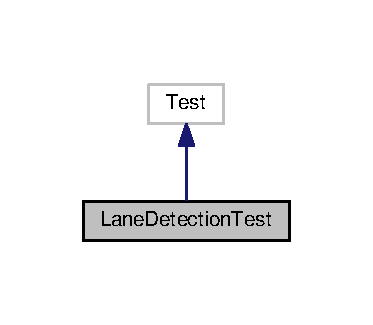
\includegraphics[width=179pt]{classLaneDetectionTest__inherit__graph}
\end{center}
\end{figure}


Collaboration diagram for Lane\+Detection\+Test\+:
\nopagebreak
\begin{figure}[H]
\begin{center}
\leavevmode
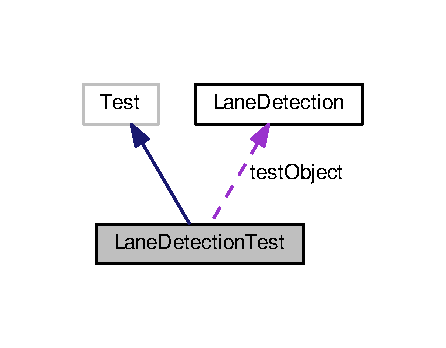
\includegraphics[width=214pt]{classLaneDetectionTest__coll__graph}
\end{center}
\end{figure}
\subsection*{Protected Attributes}
\begin{DoxyCompactItemize}
\item 
\hyperlink{classLaneDetection}{Lane\+Detection} {\bfseries test\+Object}\hypertarget{classLaneDetectionTest_a6b2e5e966d2d3b19b8389608a08657af}{}\label{classLaneDetectionTest_a6b2e5e966d2d3b19b8389608a08657af}

\end{DoxyCompactItemize}


\subsection{Detailed Description}
Class to test \hyperlink{classLaneDetection}{Lane\+Detection}. 

The documentation for this class was generated from the following file\+:\begin{DoxyCompactItemize}
\item 
/home/akash/\+Lane\+Detection\+\_\+master/\+Lane\+Detection\+System/test/\hyperlink{LaneDetectionTest_8cpp}{Lane\+Detection\+Test.\+cpp}\end{DoxyCompactItemize}

\hypertarget{classLaneInfo}{}\section{Lane\+Info Class Reference}
\label{classLaneInfo}\index{Lane\+Info@{Lane\+Info}}
\subsection*{Public Member Functions}
\begin{DoxyCompactItemize}
\item 
\hyperlink{classLaneInfo_ae4456324bd7c15c1848d0dd6dea53b4d}{Lane\+Info} ()
\begin{DoxyCompactList}\small\item\em Default constructor for \hyperlink{classLaneDetection}{Lane\+Detection}. \end{DoxyCompactList}\item 
\hyperlink{classLaneInfo_a9dd2b4e25bd67b27c65b54aced06cee4}{$\sim$\+Lane\+Info} ()
\begin{DoxyCompactList}\small\item\em Default destructor for \hyperlink{classLaneDetection}{Lane\+Detection}. \end{DoxyCompactList}\item 
void \hyperlink{classLaneInfo_a39946db06ad80f1b5f1a94f8fe81393e}{set\+Lane\+Points} (std\+::vector$<$ cv\+::\+Point $>$ lane\+Points)
\begin{DoxyCompactList}\small\item\em Function to set lane\+Points. \end{DoxyCompactList}\item 
void \hyperlink{classLaneInfo_a1ae9fe2b711ae9dfbf9f3d167254a844}{set\+Lane\+Coeffs} (cv\+::\+Mat lane\+Coeffs)
\begin{DoxyCompactList}\small\item\em Function to set lane\+Coeffs. \end{DoxyCompactList}\item 
void \hyperlink{classLaneInfo_a1e362dd10c9c25eaa74f45f3eec47fdd}{set\+Lane\+Color} (cv\+::\+Vec3b lane\+Color)
\begin{DoxyCompactList}\small\item\em Function to set lane\+Color. \end{DoxyCompactList}\item 
std\+::vector$<$ cv\+::\+Point $>$ \hyperlink{classLaneInfo_a548666413272e1a4bb09950ba15fb48b}{get\+Lane\+Points} (void)
\begin{DoxyCompactList}\small\item\em Function to get lane\+Points. \end{DoxyCompactList}\item 
cv\+::\+Mat \hyperlink{classLaneInfo_a1796822568a6ca00a291cff150ef607e}{get\+Lane\+Coeffs} (void)
\begin{DoxyCompactList}\small\item\em Function to get lane\+Coeffs. \end{DoxyCompactList}\item 
cv\+::\+Vec3b \hyperlink{classLaneInfo_a83d541beb6728ae03551293b659c6c9d}{get\+Lane\+Color} (void)
\begin{DoxyCompactList}\small\item\em Function to get lane\+Color. \end{DoxyCompactList}\end{DoxyCompactItemize}


\subsection{Constructor \& Destructor Documentation}
\index{Lane\+Info@{Lane\+Info}!Lane\+Info@{Lane\+Info}}
\index{Lane\+Info@{Lane\+Info}!Lane\+Info@{Lane\+Info}}
\subsubsection[{\texorpdfstring{Lane\+Info()}{LaneInfo()}}]{\setlength{\rightskip}{0pt plus 5cm}Lane\+Info\+::\+Lane\+Info (
\begin{DoxyParamCaption}
{}
\end{DoxyParamCaption}
)}\hypertarget{classLaneInfo_ae4456324bd7c15c1848d0dd6dea53b4d}{}\label{classLaneInfo_ae4456324bd7c15c1848d0dd6dea53b4d}


Default constructor for \hyperlink{classLaneDetection}{Lane\+Detection}. 


\begin{DoxyParams}{Parameters}
{\em nothing} & \\
\hline
\end{DoxyParams}
\begin{DoxyReturn}{Returns}
nothing 
\end{DoxyReturn}
\index{Lane\+Info@{Lane\+Info}!````~Lane\+Info@{$\sim$\+Lane\+Info}}
\index{````~Lane\+Info@{$\sim$\+Lane\+Info}!Lane\+Info@{Lane\+Info}}
\subsubsection[{\texorpdfstring{$\sim$\+Lane\+Info()}{~LaneInfo()}}]{\setlength{\rightskip}{0pt plus 5cm}Lane\+Info\+::$\sim$\+Lane\+Info (
\begin{DoxyParamCaption}
{}
\end{DoxyParamCaption}
)}\hypertarget{classLaneInfo_a9dd2b4e25bd67b27c65b54aced06cee4}{}\label{classLaneInfo_a9dd2b4e25bd67b27c65b54aced06cee4}


Default destructor for \hyperlink{classLaneDetection}{Lane\+Detection}. 


\begin{DoxyParams}{Parameters}
{\em nothing} & \\
\hline
\end{DoxyParams}
\begin{DoxyReturn}{Returns}
nothing 
\end{DoxyReturn}


\subsection{Member Function Documentation}
\index{Lane\+Info@{Lane\+Info}!get\+Lane\+Coeffs@{get\+Lane\+Coeffs}}
\index{get\+Lane\+Coeffs@{get\+Lane\+Coeffs}!Lane\+Info@{Lane\+Info}}
\subsubsection[{\texorpdfstring{get\+Lane\+Coeffs(void)}{getLaneCoeffs(void)}}]{\setlength{\rightskip}{0pt plus 5cm}cv\+::\+Mat Lane\+Info\+::get\+Lane\+Coeffs (
\begin{DoxyParamCaption}
\item[{void}]{}
\end{DoxyParamCaption}
)}\hypertarget{classLaneInfo_a1796822568a6ca00a291cff150ef607e}{}\label{classLaneInfo_a1796822568a6ca00a291cff150ef607e}


Function to get lane\+Coeffs. 


\begin{DoxyParams}{Parameters}
{\em nothing} & \\
\hline
\end{DoxyParams}
\begin{DoxyReturn}{Returns}
lane coefficients of type cv\+::\+Mat 
\end{DoxyReturn}
\index{Lane\+Info@{Lane\+Info}!get\+Lane\+Color@{get\+Lane\+Color}}
\index{get\+Lane\+Color@{get\+Lane\+Color}!Lane\+Info@{Lane\+Info}}
\subsubsection[{\texorpdfstring{get\+Lane\+Color(void)}{getLaneColor(void)}}]{\setlength{\rightskip}{0pt plus 5cm}cv\+::\+Vec3b Lane\+Info\+::get\+Lane\+Color (
\begin{DoxyParamCaption}
\item[{void}]{}
\end{DoxyParamCaption}
)}\hypertarget{classLaneInfo_a83d541beb6728ae03551293b659c6c9d}{}\label{classLaneInfo_a83d541beb6728ae03551293b659c6c9d}


Function to get lane\+Color. 


\begin{DoxyParams}{Parameters}
{\em nothing} & \\
\hline
\end{DoxyParams}
\begin{DoxyReturn}{Returns}
lane color of type cv\+::\+Vec3b 
\end{DoxyReturn}
\index{Lane\+Info@{Lane\+Info}!get\+Lane\+Points@{get\+Lane\+Points}}
\index{get\+Lane\+Points@{get\+Lane\+Points}!Lane\+Info@{Lane\+Info}}
\subsubsection[{\texorpdfstring{get\+Lane\+Points(void)}{getLanePoints(void)}}]{\setlength{\rightskip}{0pt plus 5cm}std\+::vector$<$ cv\+::\+Point $>$ Lane\+Info\+::get\+Lane\+Points (
\begin{DoxyParamCaption}
\item[{void}]{}
\end{DoxyParamCaption}
)}\hypertarget{classLaneInfo_a548666413272e1a4bb09950ba15fb48b}{}\label{classLaneInfo_a548666413272e1a4bb09950ba15fb48b}


Function to get lane\+Points. 


\begin{DoxyParams}{Parameters}
{\em nothing} & \\
\hline
\end{DoxyParams}
\begin{DoxyReturn}{Returns}
set of lane pixels of type std\+::vector$<$cv\+::\+Point$>$ 
\end{DoxyReturn}
\index{Lane\+Info@{Lane\+Info}!set\+Lane\+Coeffs@{set\+Lane\+Coeffs}}
\index{set\+Lane\+Coeffs@{set\+Lane\+Coeffs}!Lane\+Info@{Lane\+Info}}
\subsubsection[{\texorpdfstring{set\+Lane\+Coeffs(cv\+::\+Mat lane\+Coeffs)}{setLaneCoeffs(cv::Mat laneCoeffs)}}]{\setlength{\rightskip}{0pt plus 5cm}void Lane\+Info\+::set\+Lane\+Coeffs (
\begin{DoxyParamCaption}
\item[{cv\+::\+Mat}]{lane\+Coeffs}
\end{DoxyParamCaption}
)}\hypertarget{classLaneInfo_a1ae9fe2b711ae9dfbf9f3d167254a844}{}\label{classLaneInfo_a1ae9fe2b711ae9dfbf9f3d167254a844}


Function to set lane\+Coeffs. 


\begin{DoxyParams}{Parameters}
{\em lane} & coefficients of type cv\+::\+Mat \\
\hline
\end{DoxyParams}
\begin{DoxyReturn}{Returns}
nothing 
\end{DoxyReturn}
\index{Lane\+Info@{Lane\+Info}!set\+Lane\+Color@{set\+Lane\+Color}}
\index{set\+Lane\+Color@{set\+Lane\+Color}!Lane\+Info@{Lane\+Info}}
\subsubsection[{\texorpdfstring{set\+Lane\+Color(cv\+::\+Vec3b lane\+Color)}{setLaneColor(cv::Vec3b laneColor)}}]{\setlength{\rightskip}{0pt plus 5cm}void Lane\+Info\+::set\+Lane\+Color (
\begin{DoxyParamCaption}
\item[{cv\+::\+Vec3b}]{lane\+Color}
\end{DoxyParamCaption}
)}\hypertarget{classLaneInfo_a1e362dd10c9c25eaa74f45f3eec47fdd}{}\label{classLaneInfo_a1e362dd10c9c25eaa74f45f3eec47fdd}


Function to set lane\+Color. 


\begin{DoxyParams}{Parameters}
{\em lane} & color of type cv\+::\+Vec3b \\
\hline
\end{DoxyParams}
\begin{DoxyReturn}{Returns}
nothing 
\end{DoxyReturn}
\index{Lane\+Info@{Lane\+Info}!set\+Lane\+Points@{set\+Lane\+Points}}
\index{set\+Lane\+Points@{set\+Lane\+Points}!Lane\+Info@{Lane\+Info}}
\subsubsection[{\texorpdfstring{set\+Lane\+Points(std\+::vector$<$ cv\+::\+Point $>$ lane\+Points)}{setLanePoints(std::vector< cv::Point > lanePoints)}}]{\setlength{\rightskip}{0pt plus 5cm}void Lane\+Info\+::set\+Lane\+Points (
\begin{DoxyParamCaption}
\item[{std\+::vector$<$ cv\+::\+Point $>$}]{lane\+Points}
\end{DoxyParamCaption}
)}\hypertarget{classLaneInfo_a39946db06ad80f1b5f1a94f8fe81393e}{}\label{classLaneInfo_a39946db06ad80f1b5f1a94f8fe81393e}


Function to set lane\+Points. 


\begin{DoxyParams}{Parameters}
{\em set} & of lane pixels of type std\+::vector$<$cv\+::\+Point$>$ \\
\hline
\end{DoxyParams}
\begin{DoxyReturn}{Returns}
nothing 
\end{DoxyReturn}


The documentation for this class was generated from the following files\+:\begin{DoxyCompactItemize}
\item 
/home/akash/\+Lane\+Detection\+\_\+master/\+Lane\+Detection\+System/include/Lane\+Info.\+hpp\item 
/home/akash/\+Lane\+Detection\+\_\+master/\+Lane\+Detection\+System/app/Lane\+Info.\+cpp\end{DoxyCompactItemize}

\hypertarget{classLaneInfoTest}{}\section{Lane\+Info\+Test Class Reference}
\label{classLaneInfoTest}\index{Lane\+Info\+Test@{Lane\+Info\+Test}}


Class to test \hyperlink{classLaneInfo}{Lane\+Info}.  




Inheritance diagram for Lane\+Info\+Test\+:
\nopagebreak
\begin{figure}[H]
\begin{center}
\leavevmode
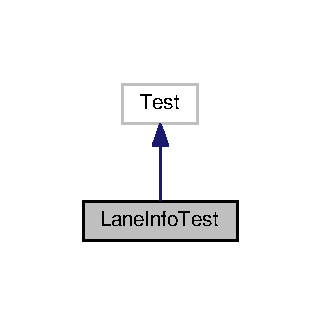
\includegraphics[width=154pt]{classLaneInfoTest__inherit__graph}
\end{center}
\end{figure}


Collaboration diagram for Lane\+Info\+Test\+:
\nopagebreak
\begin{figure}[H]
\begin{center}
\leavevmode
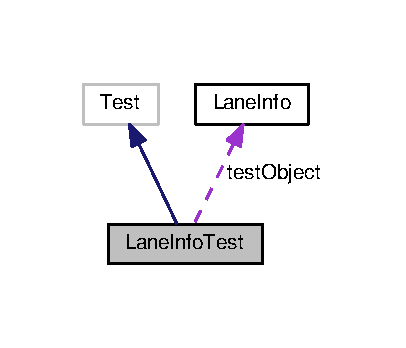
\includegraphics[width=195pt]{classLaneInfoTest__coll__graph}
\end{center}
\end{figure}
\subsection*{Protected Attributes}
\begin{DoxyCompactItemize}
\item 
\hyperlink{classLaneInfo}{Lane\+Info} {\bfseries test\+Object}\hypertarget{classLaneInfoTest_af4d53427a1f10dbc4b6668513e6febc8}{}\label{classLaneInfoTest_af4d53427a1f10dbc4b6668513e6febc8}

\end{DoxyCompactItemize}


\subsection{Detailed Description}
Class to test \hyperlink{classLaneInfo}{Lane\+Info}. 

The documentation for this class was generated from the following file\+:\begin{DoxyCompactItemize}
\item 
/home/akash/\+Lane\+Detection\+\_\+master/\+Lane\+Detection\+System/test/Lane\+Info\+Test.\+cpp\end{DoxyCompactItemize}

\chapter{File Documentation}
\hypertarget{ImageProcessing_8cpp}{}\section{/home/akash/\+Lane\+Detection\+\_\+master/\+Lane\+Detection\+System/app/\+Image\+Processing.cpp File Reference}
\label{ImageProcessing_8cpp}\index{/home/akash/\+Lane\+Detection\+\_\+master/\+Lane\+Detection\+System/app/\+Image\+Processing.\+cpp@{/home/akash/\+Lane\+Detection\+\_\+master/\+Lane\+Detection\+System/app/\+Image\+Processing.\+cpp}}


Image Processing Class File.  


{\ttfamily \#include \char`\"{}Image\+Processing.\+hpp\char`\"{}}\\*
Include dependency graph for Image\+Processing.\+cpp\+:
\nopagebreak
\begin{figure}[H]
\begin{center}
\leavevmode
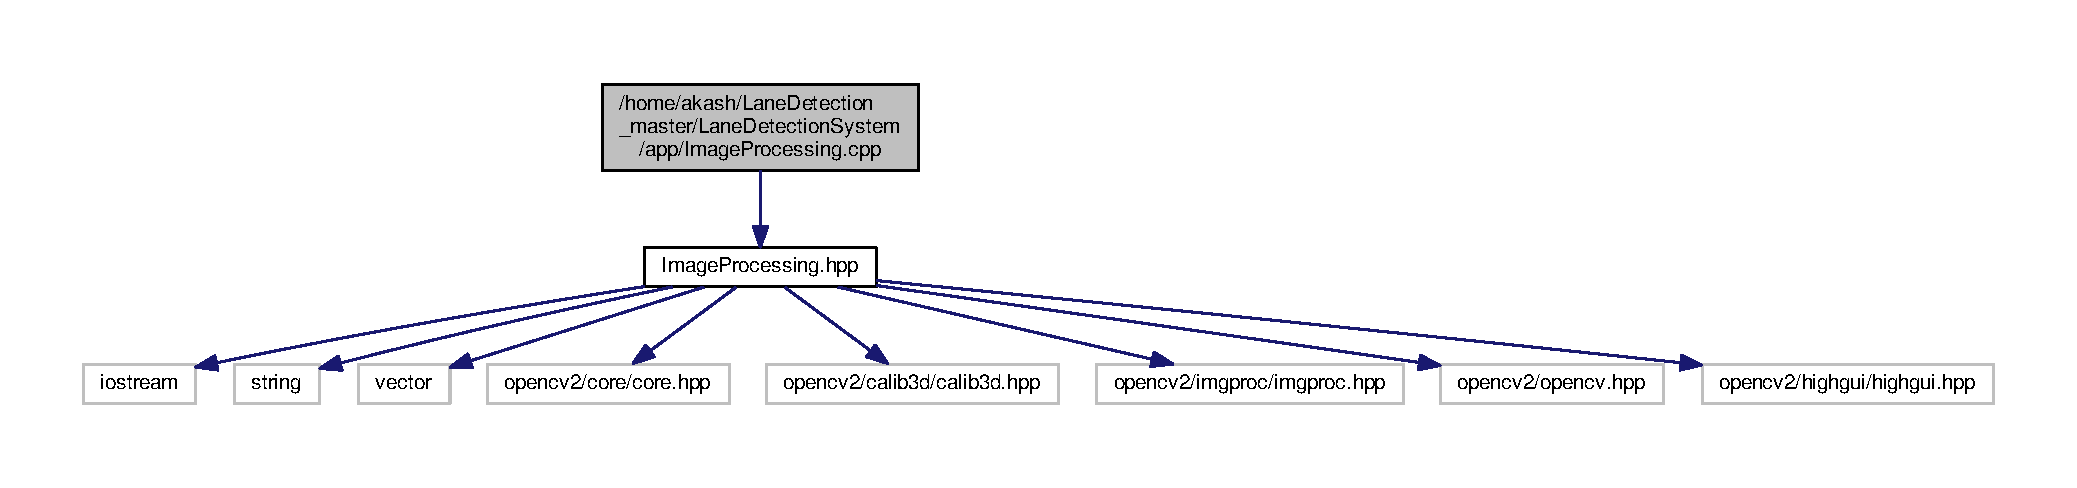
\includegraphics[width=350pt]{ImageProcessing_8cpp__incl}
\end{center}
\end{figure}
This graph shows which files directly or indirectly include this file\+:
\nopagebreak
\begin{figure}[H]
\begin{center}
\leavevmode
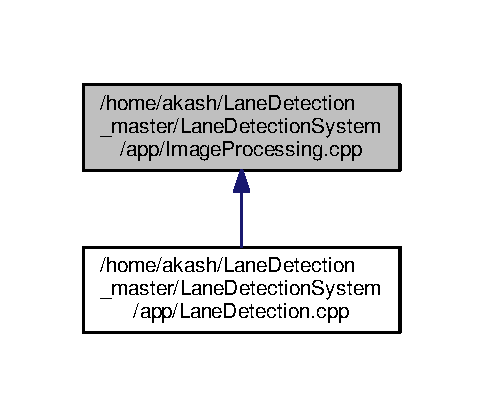
\includegraphics[width=232pt]{ImageProcessing_8cpp__dep__incl}
\end{center}
\end{figure}


\subsection{Detailed Description}
Image Processing Class File. 

Copyright \mbox{[}2018\mbox{]} rohithjayarajan, Akash Guha

\begin{DoxyAuthor}{Author}
rohithjayarajan, Akash Guha 
\end{DoxyAuthor}
\begin{DoxyDate}{Date}
10/13/2018 
\end{DoxyDate}
\begin{DoxyVersion}{Version}
1.\+1
\end{DoxyVersion}
\hypertarget{LaneDetectionTest_8cpp_DESCRIPTION}{}\subsection{D\+E\+S\+C\+R\+I\+P\+T\+I\+ON}\label{LaneDetectionTest_8cpp_DESCRIPTION}
Includes all operations for image processing and pre processing tasks to be performed on the frames in the lane detection pipeline.

Copyright \mbox{[}2018\mbox{]} rohithjayarajan, Akash Guha

\begin{DoxyAuthor}{Author}
rohithjayarajan, Akash Guha 
\end{DoxyAuthor}
\begin{DoxyDate}{Date}
10/15/2018 
\end{DoxyDate}
\begin{DoxyVersion}{Version}
1.\+1
\end{DoxyVersion}
\hypertarget{LaneDetectionTest_8cpp_DESCRIPTION}{}\subsection{D\+E\+S\+C\+R\+I\+P\+T\+I\+ON}\label{LaneDetectionTest_8cpp_DESCRIPTION}
Includes all operations for image processing and pre processing tasks to be performed on the frames in the lane detection pipeline. 
\hypertarget{LaneDetection_8cpp}{}\section{/home/akash/\+Lane\+Detection\+\_\+master/\+Lane\+Detection\+System/app/\+Lane\+Detection.cpp File Reference}
\label{LaneDetection_8cpp}\index{/home/akash/\+Lane\+Detection\+\_\+master/\+Lane\+Detection\+System/app/\+Lane\+Detection.\+cpp@{/home/akash/\+Lane\+Detection\+\_\+master/\+Lane\+Detection\+System/app/\+Lane\+Detection.\+cpp}}


Lane Detection Class file.  


{\ttfamily \#include \char`\"{}Lane\+Detection.\+hpp\char`\"{}}\\*
{\ttfamily \#include \char`\"{}Image\+Processing.\+cpp\char`\"{}}\\*
{\ttfamily \#include \char`\"{}Lane\+Info.\+cpp\char`\"{}}\\*
Include dependency graph for Lane\+Detection.\+cpp\+:
\nopagebreak
\begin{figure}[H]
\begin{center}
\leavevmode
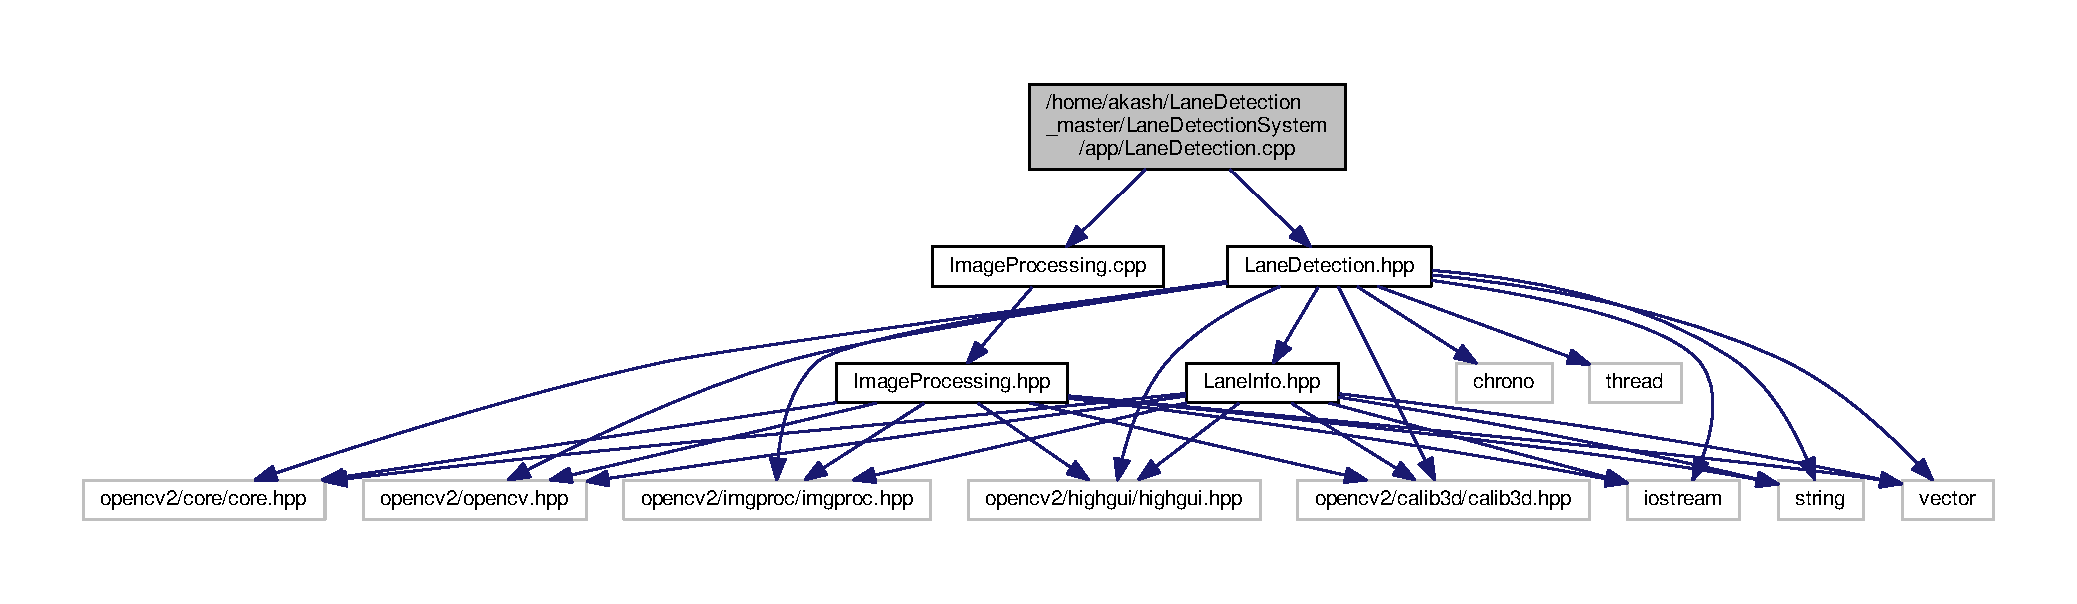
\includegraphics[width=350pt]{LaneDetection_8cpp__incl}
\end{center}
\end{figure}


\subsection{Detailed Description}
Lane Detection Class file. 

Copyright 2018 rohithjayarajan, Akash Guha

\begin{DoxyAuthor}{Author}
rohithjayarajan, Akash Guha 
\end{DoxyAuthor}
\begin{DoxyDate}{Date}
10/13/2018 
\end{DoxyDate}
\begin{DoxyVersion}{Version}
1.\+1
\end{DoxyVersion}
\hypertarget{LaneDetectionTest_8cpp_DESCRIPTION}{}\subsection{D\+E\+S\+C\+R\+I\+P\+T\+I\+ON}\label{LaneDetectionTest_8cpp_DESCRIPTION}
Class for lane detection. This includes definitions all functionalities to implement a lane detection system and to predict steering information for the vehicle. 
\hypertarget{ImageProcessing_8hpp}{}\section{/home/akash/\+Lane\+Detection\+\_\+master/\+Lane\+Detection\+System/include/\+Image\+Processing.hpp File Reference}
\label{ImageProcessing_8hpp}\index{/home/akash/\+Lane\+Detection\+\_\+master/\+Lane\+Detection\+System/include/\+Image\+Processing.\+hpp@{/home/akash/\+Lane\+Detection\+\_\+master/\+Lane\+Detection\+System/include/\+Image\+Processing.\+hpp}}


Image Processing Class Header.  


{\ttfamily \#include $<$iostream$>$}\\*
{\ttfamily \#include $<$string$>$}\\*
{\ttfamily \#include $<$vector$>$}\\*
{\ttfamily \#include \char`\"{}opencv2/core/core.\+hpp\char`\"{}}\\*
{\ttfamily \#include \char`\"{}opencv2/calib3d/calib3d.\+hpp\char`\"{}}\\*
{\ttfamily \#include \char`\"{}opencv2/imgproc/imgproc.\+hpp\char`\"{}}\\*
{\ttfamily \#include \char`\"{}opencv2/opencv.\+hpp\char`\"{}}\\*
{\ttfamily \#include \char`\"{}opencv2/highgui/highgui.\+hpp\char`\"{}}\\*
Include dependency graph for Image\+Processing.\+hpp\+:
\nopagebreak
\begin{figure}[H]
\begin{center}
\leavevmode
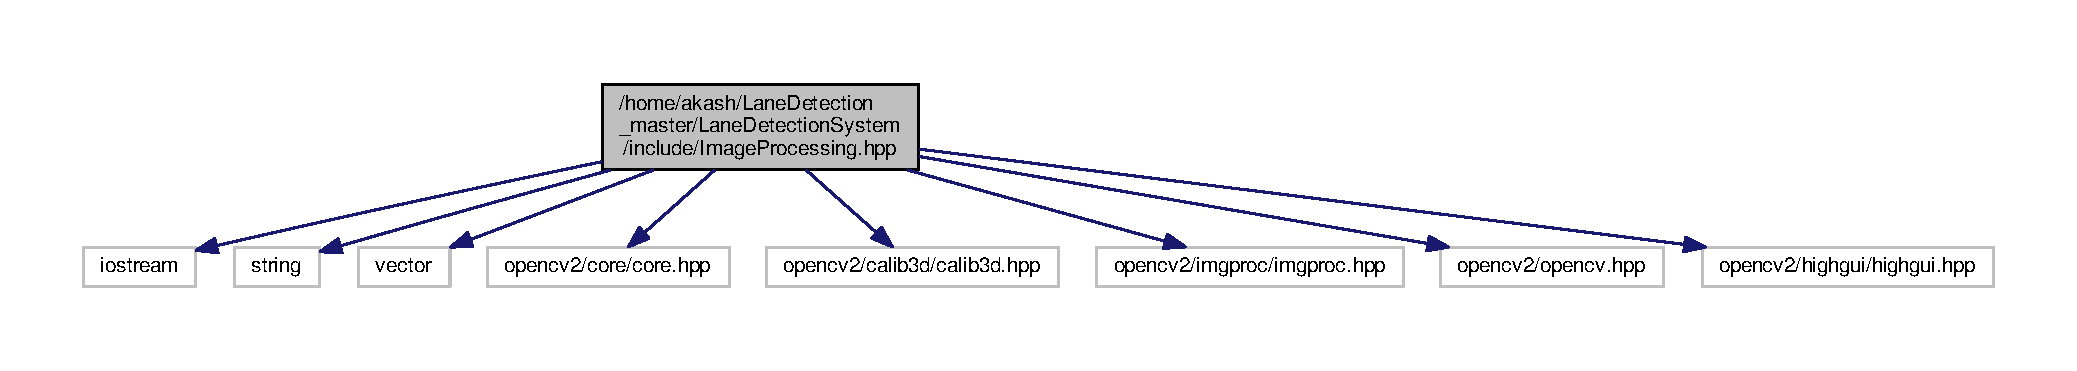
\includegraphics[width=350pt]{ImageProcessing_8hpp__incl}
\end{center}
\end{figure}
This graph shows which files directly or indirectly include this file\+:
\nopagebreak
\begin{figure}[H]
\begin{center}
\leavevmode
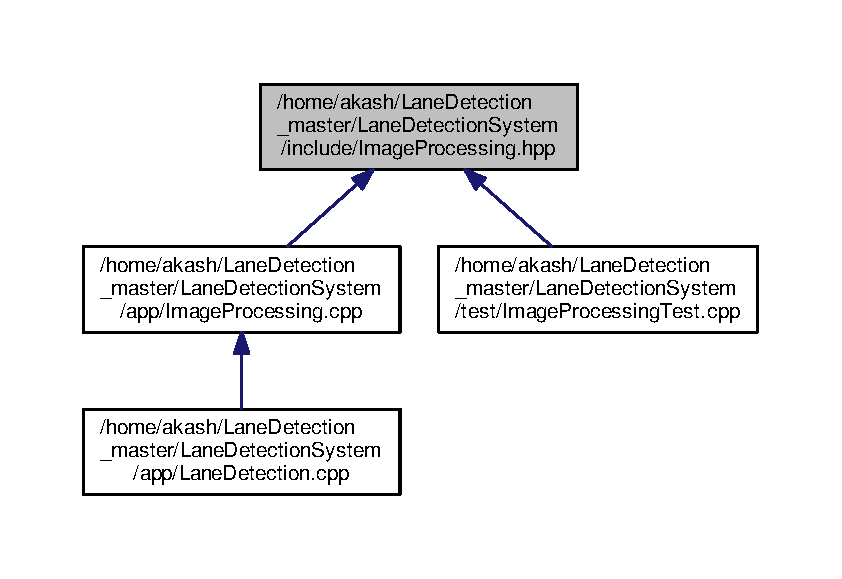
\includegraphics[width=350pt]{ImageProcessing_8hpp__dep__incl}
\end{center}
\end{figure}
\subsection*{Classes}
\begin{DoxyCompactItemize}
\item 
class \hyperlink{classImageProcessing}{Image\+Processing}
\end{DoxyCompactItemize}


\subsection{Detailed Description}
Image Processing Class Header. 

Copyright 2018 rohithjayarajan, Akash Guha

\begin{DoxyAuthor}{Author}
rohithjayarajan, Akash Guha 
\end{DoxyAuthor}
\begin{DoxyDate}{Date}
10/13/2018 
\end{DoxyDate}
\begin{DoxyVersion}{Version}
1.\+1
\end{DoxyVersion}
\hypertarget{LaneDetectionTest_8cpp_DESCRIPTION}{}\subsection{D\+E\+S\+C\+R\+I\+P\+T\+I\+ON}\label{LaneDetectionTest_8cpp_DESCRIPTION}
Class header which includes declarations of all image pre-\/processing functionalities in lane detection and steering system. 
\hypertarget{LaneDetection_8hpp}{}\section{/home/akash/\+Lane\+Detection\+\_\+master/\+Lane\+Detection\+System/include/\+Lane\+Detection.hpp File Reference}
\label{LaneDetection_8hpp}\index{/home/akash/\+Lane\+Detection\+\_\+master/\+Lane\+Detection\+System/include/\+Lane\+Detection.\+hpp@{/home/akash/\+Lane\+Detection\+\_\+master/\+Lane\+Detection\+System/include/\+Lane\+Detection.\+hpp}}


Lane Detection Class Header.  


{\ttfamily \#include $<$iostream$>$}\\*
{\ttfamily \#include $<$string$>$}\\*
{\ttfamily \#include $<$vector$>$}\\*
{\ttfamily \#include $<$chrono$>$}\\*
{\ttfamily \#include $<$thread$>$}\\*
{\ttfamily \#include \char`\"{}opencv2/core/core.\+hpp\char`\"{}}\\*
{\ttfamily \#include \char`\"{}opencv2/calib3d/calib3d.\+hpp\char`\"{}}\\*
{\ttfamily \#include \char`\"{}opencv2/imgproc/imgproc.\+hpp\char`\"{}}\\*
{\ttfamily \#include \char`\"{}opencv2/opencv.\+hpp\char`\"{}}\\*
{\ttfamily \#include \char`\"{}opencv2/highgui/highgui.\+hpp\char`\"{}}\\*
{\ttfamily \#include \char`\"{}Lane\+Info.\+hpp\char`\"{}}\\*
Include dependency graph for Lane\+Detection.\+hpp\+:
\nopagebreak
\begin{figure}[H]
\begin{center}
\leavevmode
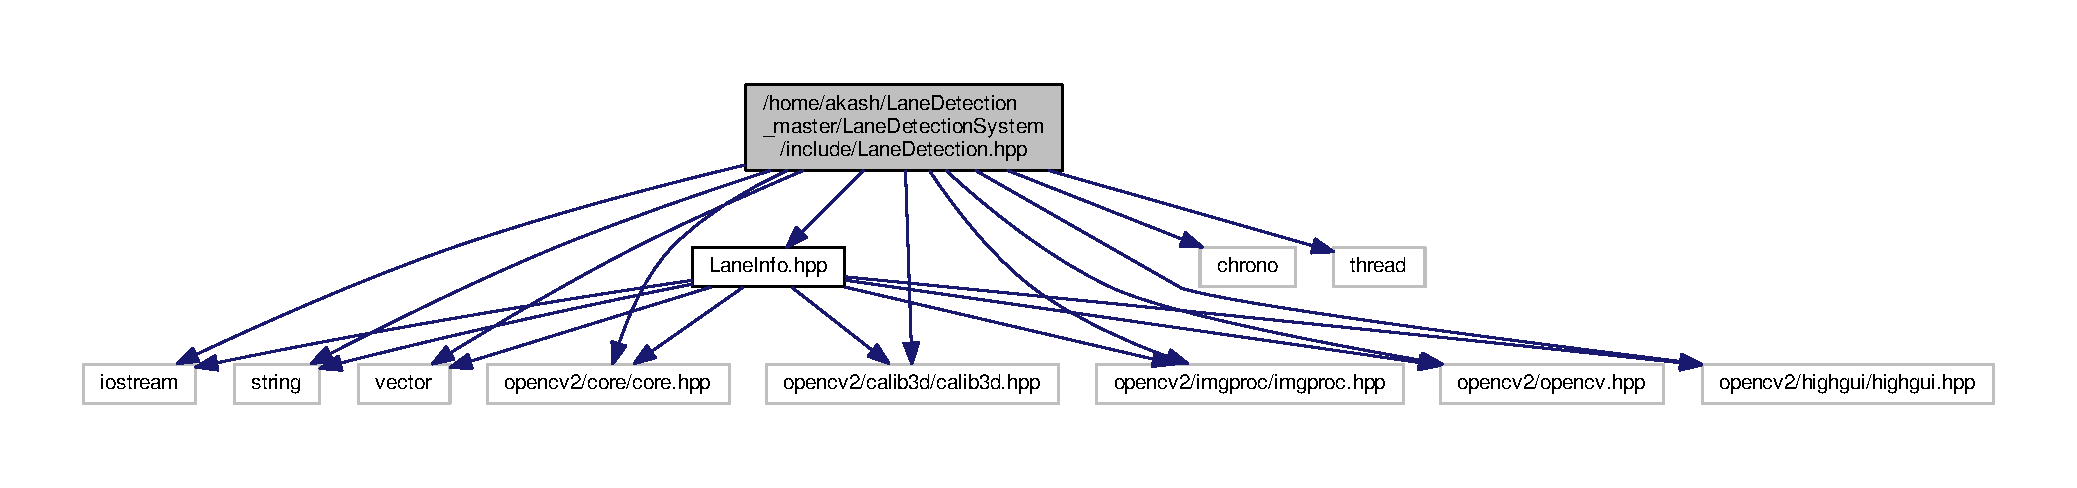
\includegraphics[width=350pt]{LaneDetection_8hpp__incl}
\end{center}
\end{figure}
This graph shows which files directly or indirectly include this file\+:
\nopagebreak
\begin{figure}[H]
\begin{center}
\leavevmode
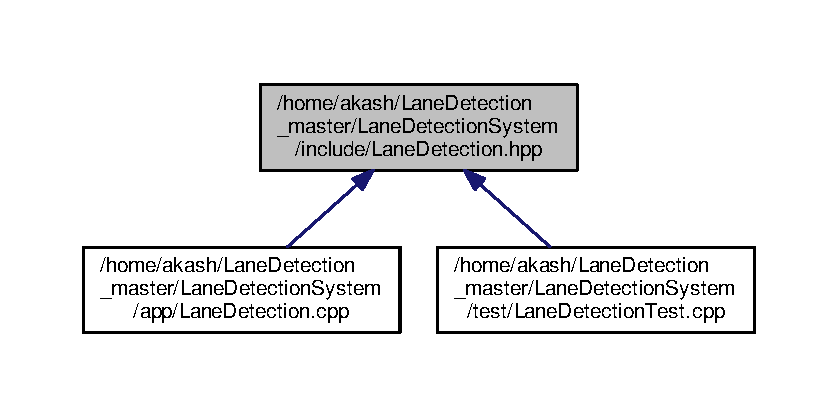
\includegraphics[width=350pt]{LaneDetection_8hpp__dep__incl}
\end{center}
\end{figure}
\subsection*{Classes}
\begin{DoxyCompactItemize}
\item 
class \hyperlink{classLaneDetection}{Lane\+Detection}
\end{DoxyCompactItemize}


\subsection{Detailed Description}
Lane Detection Class Header. 

Copyright 2018 rohithjayarajan, Akash Guha

\begin{DoxyAuthor}{Author}
rohithjayarajan, Akash Guha 
\end{DoxyAuthor}
\begin{DoxyDate}{Date}
10/13/2018 
\end{DoxyDate}
\begin{DoxyVersion}{Version}
1.\+1
\end{DoxyVersion}
\hypertarget{LaneDetectionTest_8cpp_DESCRIPTION}{}\subsection{D\+E\+S\+C\+R\+I\+P\+T\+I\+ON}\label{LaneDetectionTest_8cpp_DESCRIPTION}
Class for lane detection module. This includes declarations of all functionalities to implement a lane detection system and to predict steering information for the vehicle.

Copyright 2018 rohithjayarajan, Akash Guha

\begin{DoxyAuthor}{Author}
rohithjayarajan, Akash Guha 
\end{DoxyAuthor}
\begin{DoxyDate}{Date}
10/15/2018 
\end{DoxyDate}
\begin{DoxyVersion}{Version}
1.\+1
\end{DoxyVersion}
\hypertarget{LaneDetectionTest_8cpp_DESCRIPTION}{}\subsection{D\+E\+S\+C\+R\+I\+P\+T\+I\+ON}\label{LaneDetectionTest_8cpp_DESCRIPTION}
Class for lane detection module. This includes declarations of all functionalities to implement a lane detection system and to predict steering information for the vehicle. 
\hypertarget{ImageProcessingTest_8cpp}{}\section{/home/akash/\+Lane\+Detection\+\_\+master/\+Lane\+Detection\+System/test/\+Image\+Processing\+Test.cpp File Reference}
\label{ImageProcessingTest_8cpp}\index{/home/akash/\+Lane\+Detection\+\_\+master/\+Lane\+Detection\+System/test/\+Image\+Processing\+Test.\+cpp@{/home/akash/\+Lane\+Detection\+\_\+master/\+Lane\+Detection\+System/test/\+Image\+Processing\+Test.\+cpp}}


Image Processing Class Test.  


{\ttfamily \#include $<$gtest/gtest.\+h$>$}\\*
{\ttfamily \#include \char`\"{}Image\+Processing.\+hpp\char`\"{}}\\*
Include dependency graph for Image\+Processing\+Test.\+cpp\+:
\nopagebreak
\begin{figure}[H]
\begin{center}
\leavevmode
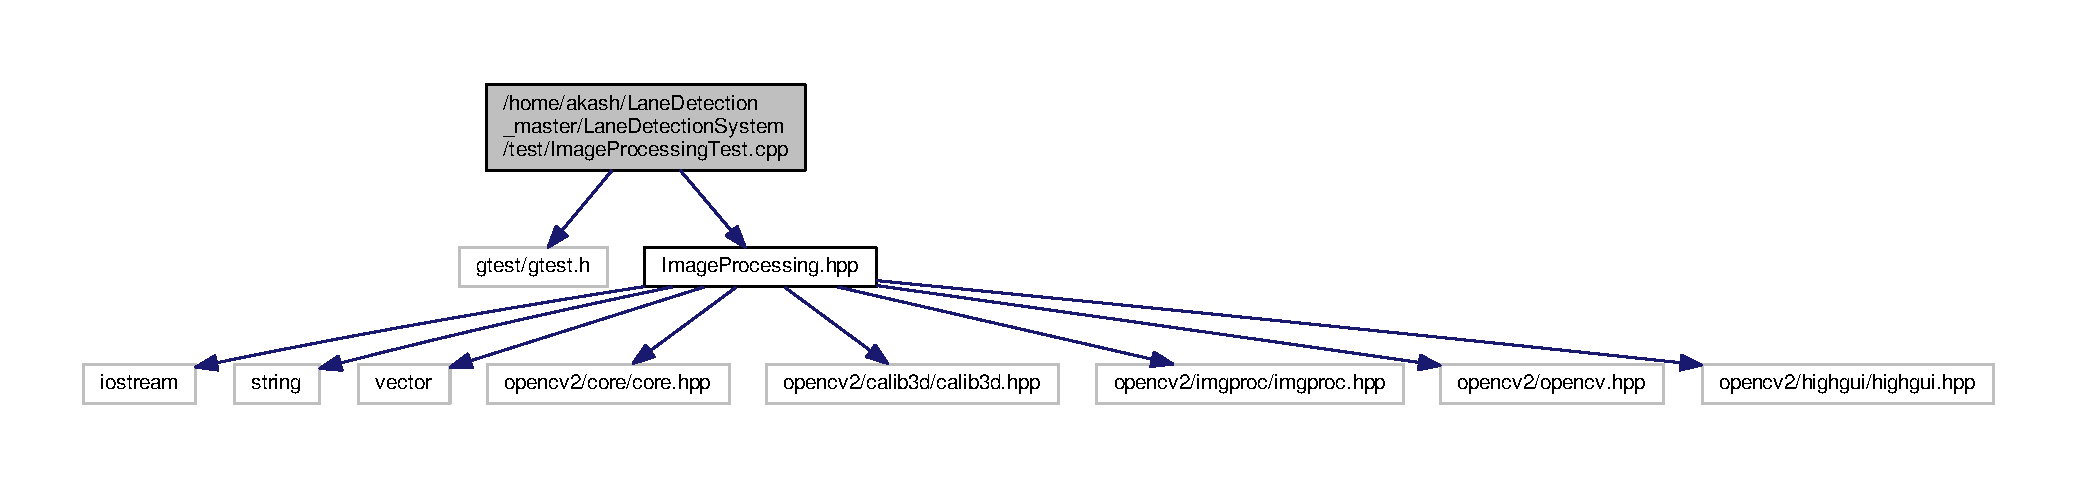
\includegraphics[width=350pt]{ImageProcessingTest_8cpp__incl}
\end{center}
\end{figure}
\subsection*{Classes}
\begin{DoxyCompactItemize}
\item 
class \hyperlink{classImageProcessingTest}{Image\+Processing\+Test}
\begin{DoxyCompactList}\small\item\em Class to test \hyperlink{classImageProcessing}{Image\+Processing}. \end{DoxyCompactList}\end{DoxyCompactItemize}
\subsection*{Functions}
\begin{DoxyCompactItemize}
\item 
\hyperlink{ImageProcessingTest_8cpp_a7ae7ec9a926a48b27f6f2dbbd54cfb43}{T\+E\+S\+T\+\_\+F} (\hyperlink{classImageProcessingTest}{Image\+Processing\+Test}, is\+Intrinsic\+Set)
\begin{DoxyCompactList}\small\item\em Test to ensure validity of pre-\/processed image. \end{DoxyCompactList}\item 
\hyperlink{ImageProcessingTest_8cpp_a142b21cb656cfe930be860a1f431c654}{T\+E\+S\+T\+\_\+F} (\hyperlink{classImageProcessingTest}{Image\+Processing\+Test}, is\+Distortion\+Coefficients\+Set)\hypertarget{ImageProcessingTest_8cpp_a142b21cb656cfe930be860a1f431c654}{}\label{ImageProcessingTest_8cpp_a142b21cb656cfe930be860a1f431c654}

\begin{DoxyCompactList}\small\item\em Test to ensure distortion coefficients are set. \end{DoxyCompactList}\item 
\hyperlink{ImageProcessingTest_8cpp_a04c792601adcba10ec43493087635acd}{T\+E\+S\+T\+\_\+F} (\hyperlink{classImageProcessingTest}{Image\+Processing\+Test}, is\+Gaussian\+Sigma\+X\+Set)\hypertarget{ImageProcessingTest_8cpp_a04c792601adcba10ec43493087635acd}{}\label{ImageProcessingTest_8cpp_a04c792601adcba10ec43493087635acd}

\begin{DoxyCompactList}\small\item\em Test to ensure standard deviation in X for gaussian blur is set. \end{DoxyCompactList}\item 
\hyperlink{ImageProcessingTest_8cpp_a39179d72411b93a4921ef0910ad44f07}{T\+E\+S\+T\+\_\+F} (\hyperlink{classImageProcessingTest}{Image\+Processing\+Test}, is\+Gaussian\+Sigma\+Y\+Set)\hypertarget{ImageProcessingTest_8cpp_a39179d72411b93a4921ef0910ad44f07}{}\label{ImageProcessingTest_8cpp_a39179d72411b93a4921ef0910ad44f07}

\begin{DoxyCompactList}\small\item\em Test to ensure standard deviation in Y for gaussian blur is set. \end{DoxyCompactList}\item 
\hyperlink{ImageProcessingTest_8cpp_a84a7d37d72c4d35837d165b39c6a5971}{T\+E\+S\+T\+\_\+F} (\hyperlink{classImageProcessingTest}{Image\+Processing\+Test}, is\+H\+S\+L\+Min\+Threshold\+Set)\hypertarget{ImageProcessingTest_8cpp_a84a7d37d72c4d35837d165b39c6a5971}{}\label{ImageProcessingTest_8cpp_a84a7d37d72c4d35837d165b39c6a5971}

\begin{DoxyCompactList}\small\item\em Test to ensure minimum threshold values of hue,saturation and luminousness are set. \end{DoxyCompactList}\item 
\hyperlink{ImageProcessingTest_8cpp_afe968709960be7bb7ee6979b0c9a5ebd}{T\+E\+S\+T\+\_\+F} (\hyperlink{classImageProcessingTest}{Image\+Processing\+Test}, is\+H\+S\+L\+Max\+Threshold\+Set)\hypertarget{ImageProcessingTest_8cpp_afe968709960be7bb7ee6979b0c9a5ebd}{}\label{ImageProcessingTest_8cpp_afe968709960be7bb7ee6979b0c9a5ebd}

\begin{DoxyCompactList}\small\item\em Test to ensure maximum threshold values of hue,saturation and luminousness are set. \end{DoxyCompactList}\item 
\hyperlink{ImageProcessingTest_8cpp_a5fb217acdb9e9c7c217b5d385a57a4c1}{T\+E\+S\+T\+\_\+F} (\hyperlink{classImageProcessingTest}{Image\+Processing\+Test}, is\+B\+G\+R\+Min\+Threshold\+Set)\hypertarget{ImageProcessingTest_8cpp_a5fb217acdb9e9c7c217b5d385a57a4c1}{}\label{ImageProcessingTest_8cpp_a5fb217acdb9e9c7c217b5d385a57a4c1}

\begin{DoxyCompactList}\small\item\em Test to ensure minimum threshold values of red, green and blue are set. \end{DoxyCompactList}\item 
\hyperlink{ImageProcessingTest_8cpp_a37708aae7c2baccc0684a6cdd4bc75c9}{T\+E\+S\+T\+\_\+F} (\hyperlink{classImageProcessingTest}{Image\+Processing\+Test}, is\+B\+G\+R\+Max\+Threshold\+Set)\hypertarget{ImageProcessingTest_8cpp_a37708aae7c2baccc0684a6cdd4bc75c9}{}\label{ImageProcessingTest_8cpp_a37708aae7c2baccc0684a6cdd4bc75c9}

\begin{DoxyCompactList}\small\item\em Test to ensure maximum threshold values of red, green and blue are set. \end{DoxyCompactList}\end{DoxyCompactItemize}


\subsection{Detailed Description}
Image Processing Class Test. 

Copyright \mbox{[}2018\mbox{]} Akash Guha

\begin{DoxyAuthor}{Author}
Akash Guha
\end{DoxyAuthor}
\hypertarget{LaneDetectionTest_8cpp_DESCRIPTION}{}\subsection{D\+E\+S\+C\+R\+I\+P\+T\+I\+ON}\label{LaneDetectionTest_8cpp_DESCRIPTION}
This module tests the functionality of the image processing class. 

\subsection{Function Documentation}
\index{Image\+Processing\+Test.\+cpp@{Image\+Processing\+Test.\+cpp}!T\+E\+S\+T\+\_\+F@{T\+E\+S\+T\+\_\+F}}
\index{T\+E\+S\+T\+\_\+F@{T\+E\+S\+T\+\_\+F}!Image\+Processing\+Test.\+cpp@{Image\+Processing\+Test.\+cpp}}
\subsubsection[{\texorpdfstring{T\+E\+S\+T\+\_\+\+F(\+Image\+Processing\+Test, is\+Intrinsic\+Set)}{TEST_F(ImageProcessingTest, isIntrinsicSet)}}]{\setlength{\rightskip}{0pt plus 5cm}T\+E\+S\+T\+\_\+F (
\begin{DoxyParamCaption}
\item[{{\bf Image\+Processing\+Test}}]{, }
\item[{is\+Intrinsic\+Set}]{}
\end{DoxyParamCaption}
)}\hypertarget{ImageProcessingTest_8cpp_a7ae7ec9a926a48b27f6f2dbbd54cfb43}{}\label{ImageProcessingTest_8cpp_a7ae7ec9a926a48b27f6f2dbbd54cfb43}


Test to ensure validity of pre-\/processed image. 

Test to ensure validity of binary thresholding Test to ensure validity of prespective transformation Test to ensure intrinsic parameters are set 
\hypertarget{LaneDetectionTest_8cpp}{}\section{/home/akash/\+Lane\+Detection\+\_\+master/\+Lane\+Detection\+System/test/\+Lane\+Detection\+Test.cpp File Reference}
\label{LaneDetectionTest_8cpp}\index{/home/akash/\+Lane\+Detection\+\_\+master/\+Lane\+Detection\+System/test/\+Lane\+Detection\+Test.\+cpp@{/home/akash/\+Lane\+Detection\+\_\+master/\+Lane\+Detection\+System/test/\+Lane\+Detection\+Test.\+cpp}}


Lane Detection Test.  


{\ttfamily \#include $<$gtest/gtest.\+h$>$}\\*
{\ttfamily \#include \char`\"{}Lane\+Detection.\+hpp\char`\"{}}\\*
Include dependency graph for Lane\+Detection\+Test.\+cpp\+:
\nopagebreak
\begin{figure}[H]
\begin{center}
\leavevmode
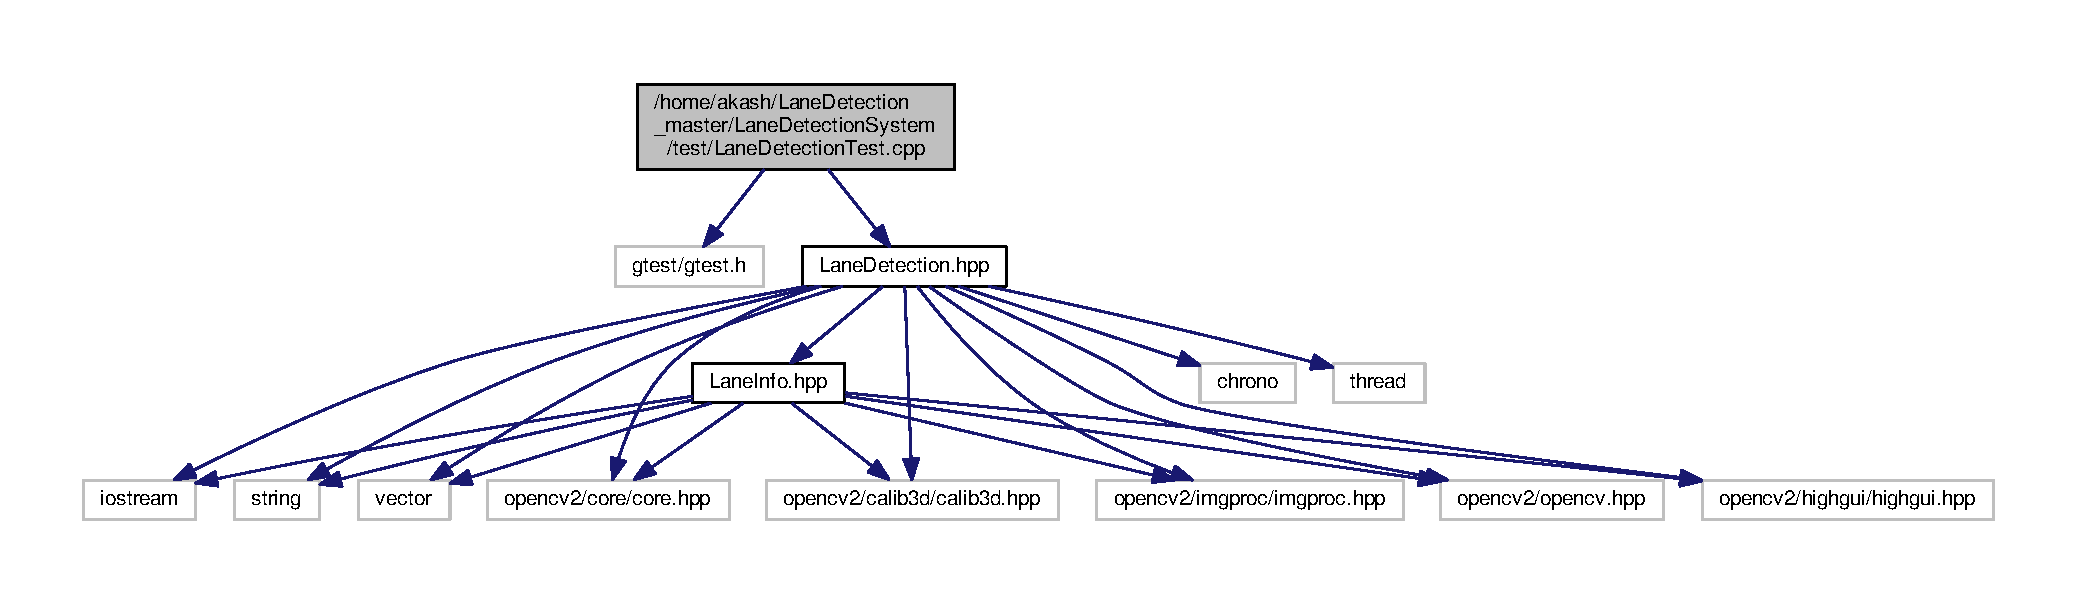
\includegraphics[width=350pt]{LaneDetectionTest_8cpp__incl}
\end{center}
\end{figure}
\subsection*{Classes}
\begin{DoxyCompactItemize}
\item 
class \hyperlink{classLaneDetectionTest}{Lane\+Detection\+Test}
\begin{DoxyCompactList}\small\item\em Class to test \hyperlink{classLaneDetection}{Lane\+Detection}. \end{DoxyCompactList}\end{DoxyCompactItemize}
\subsection*{Functions}
\begin{DoxyCompactItemize}
\item 
\hyperlink{LaneDetectionTest_8cpp_a136a530e8998ff6c16bdb03f55bd418f}{T\+E\+S\+T\+\_\+F} (\hyperlink{classLaneDetectionTest}{Lane\+Detection\+Test}, radius\+Of\+Curve\+Check)\hypertarget{LaneDetectionTest_8cpp_a136a530e8998ff6c16bdb03f55bd418f}{}\label{LaneDetectionTest_8cpp_a136a530e8998ff6c16bdb03f55bd418f}

\begin{DoxyCompactList}\small\item\em Test to check radius of curvature of lanes. \end{DoxyCompactList}\end{DoxyCompactItemize}


\subsection{Detailed Description}
Lane Detection Test. 

Copyright \mbox{[}2018\mbox{]} Akash Guha

\begin{DoxyAuthor}{Author}
Akash Guha
\end{DoxyAuthor}
\hypertarget{LaneDetectionTest_8cpp_DESCRIPTION}{}\subsection{D\+E\+S\+C\+R\+I\+P\+T\+I\+ON}\label{LaneDetectionTest_8cpp_DESCRIPTION}
This module tests the functionality of the lane detection class. 
%--- End generated contents ---

% Index
\backmatter
\newpage
\phantomsection
\clearemptydoublepage
\addcontentsline{toc}{chapter}{Index}
\printindex

\end{document}
